\documentclass[a4paper]{article}
\usepackage{graphicx} % Required for inserting images
\usepackage{polski}
\usepackage{float}
\usepackage{listings}
\usepackage{xcolor}
\usepackage{hyperref}
\usepackage{a4wide}
\usepackage{booktabs}

% Konfiguracja wyglądu kodu JSON
\colorlet{punct}{red!60!black}
\definecolor{background}{HTML}{EEEEEE}
\definecolor{delim}{RGB}{20,105,176}
\colorlet{numb}{magenta!60!black}

\lstdefinelanguage{json}{
    basicstyle=\normalfont\ttfamily,
    numbers=left,
    numberstyle=\scriptsize,
    stepnumber=1,
    numbersep=8pt,
    showstringspaces=false,
    breaklines=true,
    backgroundcolor=\color{background},
    literate=
     *{:}{{{\color{punct}{:}}}}{1}
      {,}{{{\color{punct}{,}}}}{1}
      {\{}{{{\color{delim}{\{}}}}{1}
      {\}}{{{\color{delim}{\}}}}}{1}
      {[}{{{\color{delim}{[}}}}{1}
      {]}{{{\color{delim}{]}}}}{1},
}

\lstdefinestyle{pythonStyle}{
    language=Python,
    basicstyle=\ttfamily\small,
    keywordstyle=\color{blue}\bfseries,
    commentstyle=\color{gray},
    stringstyle=\color{green!60!black},
    numbers=left,
    numberstyle=\tiny\color{gray},
    stepnumber=1,
    breaklines=true,
    showstringspaces=false,
    extendedchars=true,
    literate=
    {ą}{{\k{a}}}1 {ć}{{\'c}}1 {ę}{{\k{e}}}1 {ł}{{\l{}}}1 {ń}{{\'n}}1 {ó}{{\'o}}1 {ś}{{\'s}}1 {ź}{{\'z}}1 {ż}{{\.z}}1
    {Ą}{{\k{A}}}1 {Ć}{{\'C}}1 {Ę}{{\k{E}}}1 {Ł}{{\L{}}}1 {Ń}{{\'N}}1 {Ó}{{\'O}}1 {Ś}{{\'S}}1 {Ź}{{\'Z}}1 {Ż}{{\.Z}}1
}

\title{\textbf{Sprawozdanie z projektu}\\Zastosowanie modeli wizualno-językowych do przetwarzania sekwencji wideo nagrań ruchu drogowego}
\author{\textbf{Opiekun naukowy:} dr hab. inż. Marcin Iwanowski\\
       \textbf{ Autor:} Łukasz Jugo}
\date{\today}

\begin{document}

\maketitle
\newpage
\tableofcontents
\newpage

\section{Wstęp}
Niniejszy projekt został zrealizowany jako projekt dyplomowy na studiach inżynierskich. Obejmuje on przeprowadzenie analizy i badań nad wykorzystaniem modeli VLM (vision-language model) do przetwarzania sekwencji wideo nagrań z ruchu drogowego. Kluczowym aspektem pozwalającym na efektywne wykorzystywanie owych modeli jest selekcja fragmentów nagrań, które będą przekazywane do modelu wizualno-językowego. Jako wstęp do późniejszej pracy inżynierskiej ten projekt skupia się głównie na tym aspekcie. Przez większość czasu (szczególnie w przypadku mniej ruchliwych dróg) na obrazie z ruchu drogowego nie dzieje się nic co wymagałoby szczególnej uwagi. Z tego powodu przekazywanie wielogodzinnych nagrań do modeli jest bezcelowe i powoduje marnowanie zasobów. Sprawia to, że przed przystąpieniem do bezpośredniej analizy nagrań należy zwrócić uwagę na selekcję najbardziej interesujących fragmentów. Można wyróżnić dwa sposoby wykonania takiej czynności: manualny i automatyczny. W trybie manualnym operator systemu sam oznacza np. interesującą go linię i jeśli dany obiekt ją przekroczy sekwencja się zaczyna. W trybie automatycznym system sam na podstawie analizy odpowiednio długiego fragmentu nagrania ustala intersujący go obszar zainteresowania. W dalszej części sprawozdania przedstawiam sposób podejścia do tych problemów zaproponowany przeze mnie.
\section{Badania nad zastosowaniem detektorów obiektów do ekstrakcji kluczowych obiektów w ruchu drogowym}
Aby przystąpić do próby ekstrakcji fragmentów nagrań, przede wszystkim trzeba poruszyć kwestię detekcji obiektów na obrazach jak również ich późniejszego śledzenia w celu identyfikacji czy dany obiekt spełnił nasze kryteria zainteresowania.
\subsection{Tryb manualny}
W trybie manualnym przeanalizowałem dwie możliwości wykrywania obiektów:
\begin{itemize}
    \item kaskady Haara - ich zaletą jest niewątpliwie prostota i niska złożoność obliczeniowa, a wadami problemy z detekcją przy słabych warunkach oświetleniowych oraz brak informacji o klasie obiektu
    \item sieć neuronowa YOLO - jej ogromną zaletą jest wbudowana opcja trackingu, automatyczna klasyfikacja i różnorodność wersji pozwalających dostosować poziom zaawansowania sieci do możliwości maszyny, natomiast jej wadą są niewątpliwie wymagania sprzętowe szczególnie w przypadku większych modeli (np. wersji X czy L).
\end{itemize}
Stworzone zostały dwa proste programy \textit{wykrywanie\_haar.py} i \textit{wykrywanie\_yolo.py}. Oba te programy w kwestii śledzenia obiektów opierają się na bardzo prostym trackerze centoridowym inspirowanym klasyczną metodą klasyfikacji k-najbliższych sąsiadów.
Na początku operator musi zaznaczyć linię, której przekroczenie badał będzie program.
\begin{figure}[H]
    \centering
    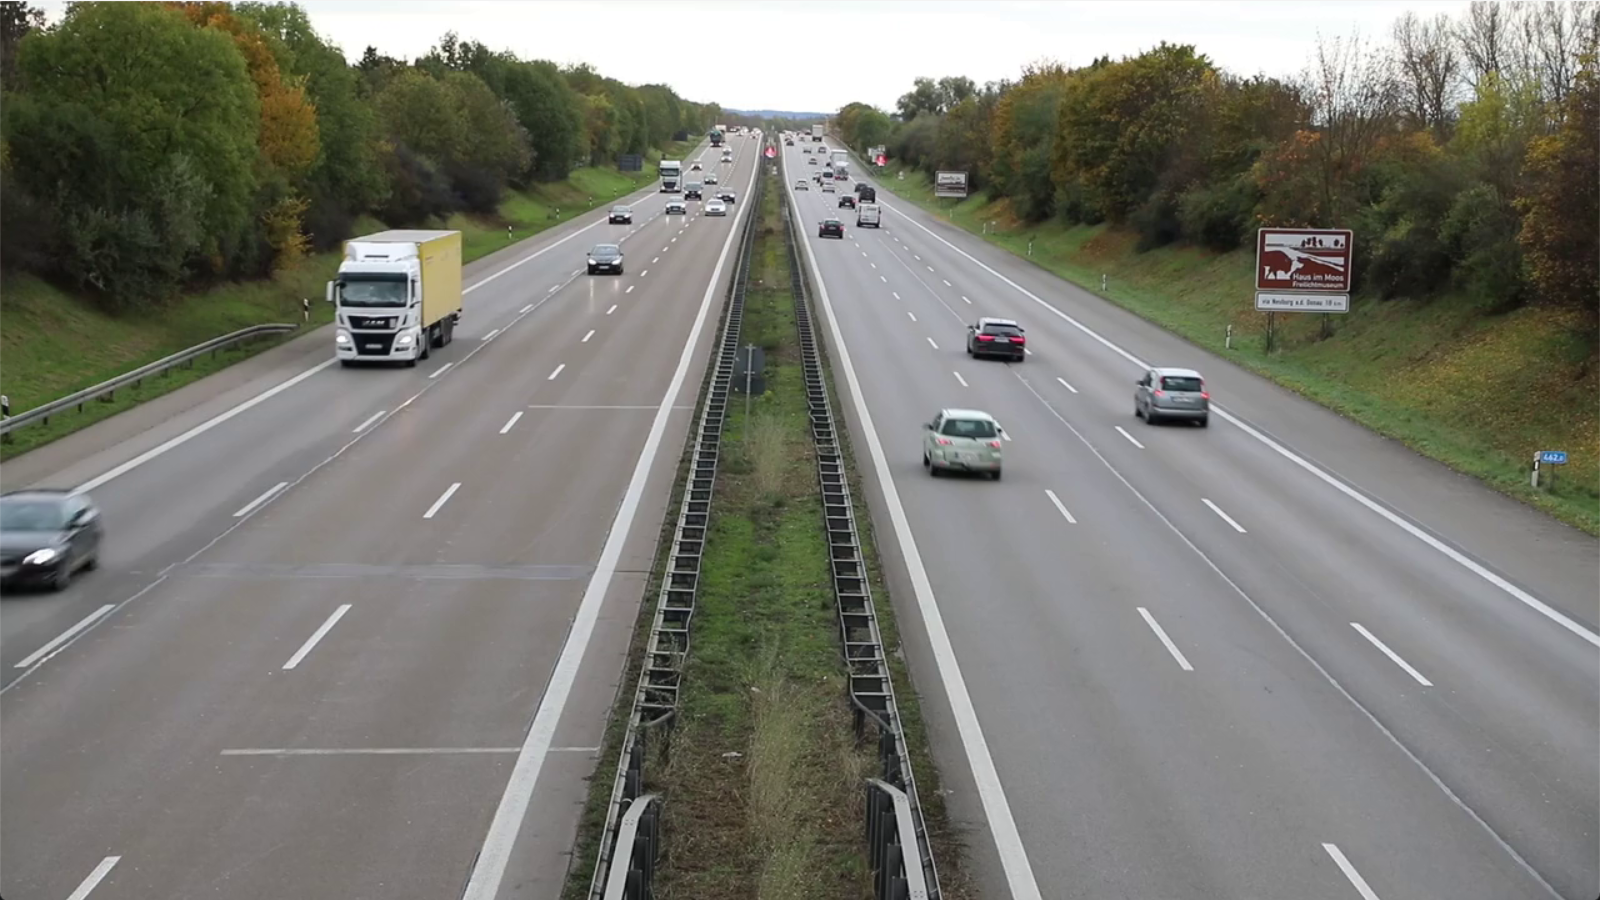
\includegraphics[width=0.95\textwidth]{images/manual1.png}
    \caption{Program w trybie startowym przed narysowaniem linii przez operatora}
\end{figure}
\begin{figure}[H]
    \centering
    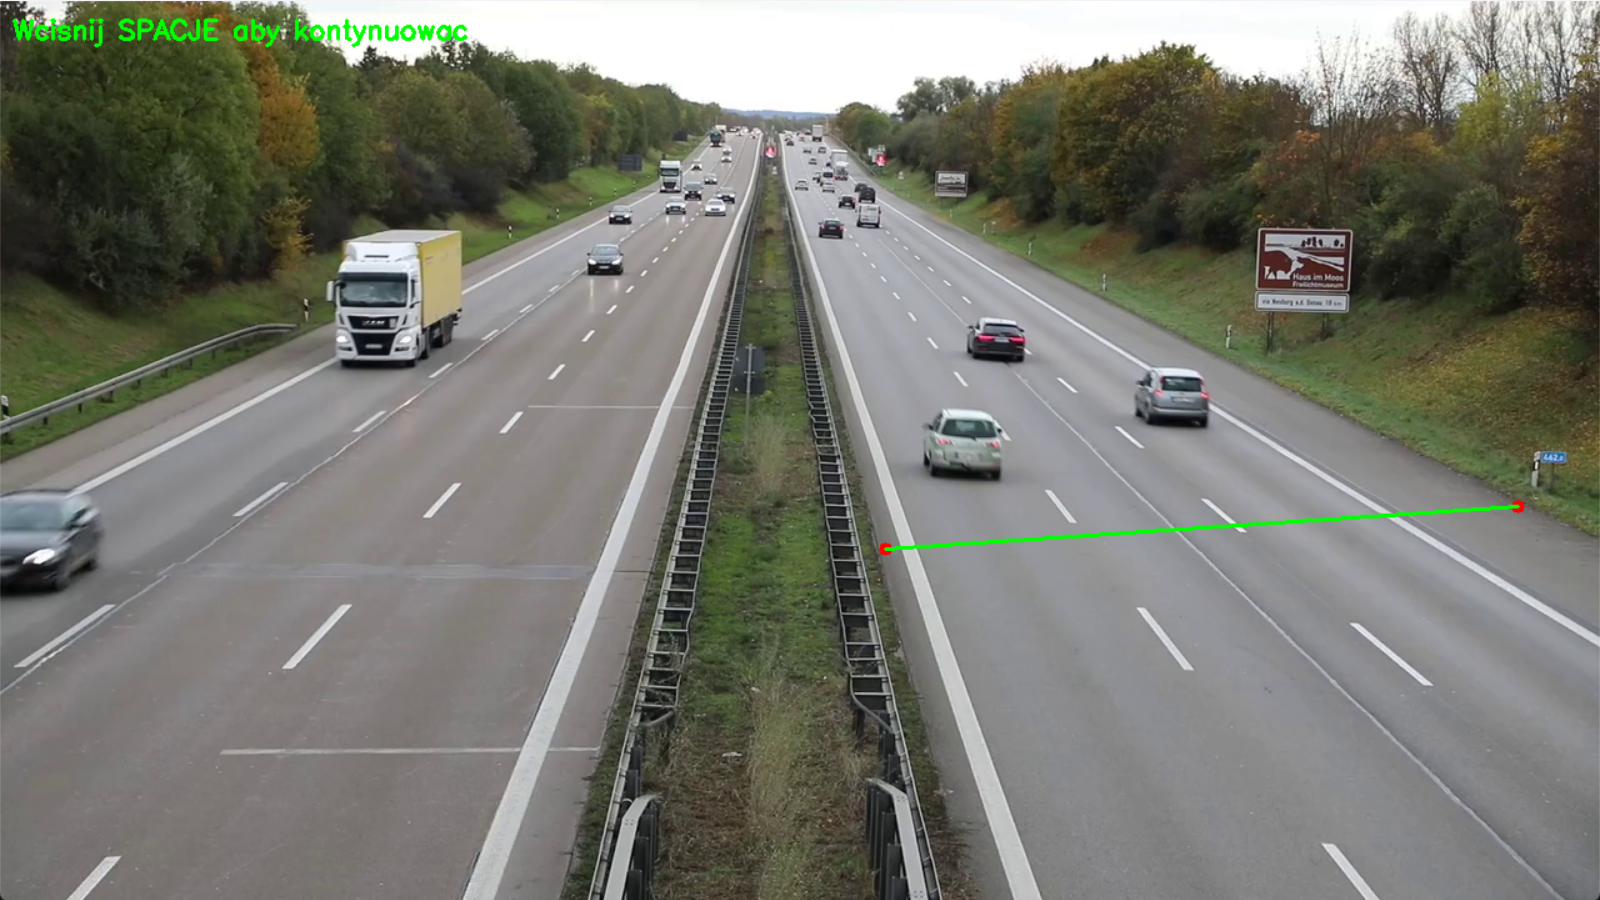
\includegraphics[width=0.95\textwidth]{images/manual2.png}
    \caption{Program w trybie startowym po narysowaniu linii przez operatora}
\end{figure}
Po wciśnięciu spacji rozpoczyna się wykrywanie. Przejście obiektu przez linię analizowane jest za pomocą iloczynu wektorowego dwóch wektorów rozpiętych na następujących punktach: centroid obiektu, początek linii, koniec linii. Jeśli wykryta zostana zmiana znaku w iloczynie uznaje się, że obiekt przekroczył linię. Informację o tym operator dostaje w formie tekstu wypisanego w terminalu.
\begin{figure}[H]
    \centering
    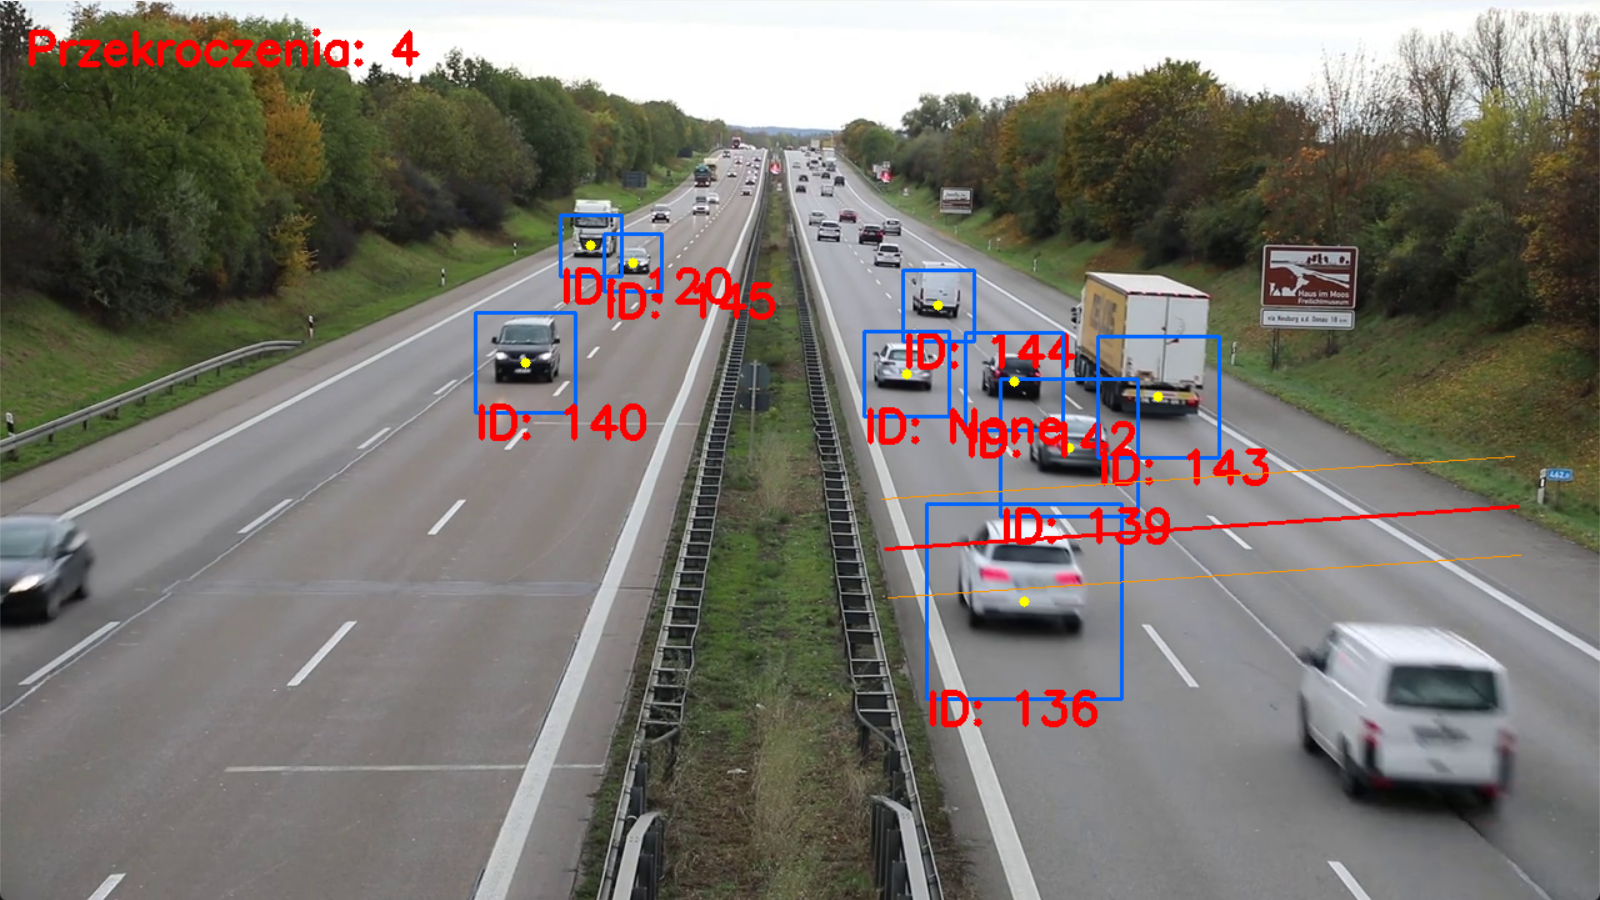
\includegraphics[width=0.95\textwidth]{images/manual3.png}
    \caption{Program w trakcie wykrywania obiektów i przekroczenia przez nie wyznaczonej linii}
\end{figure}
\begin{figure}[H]
    \centering
    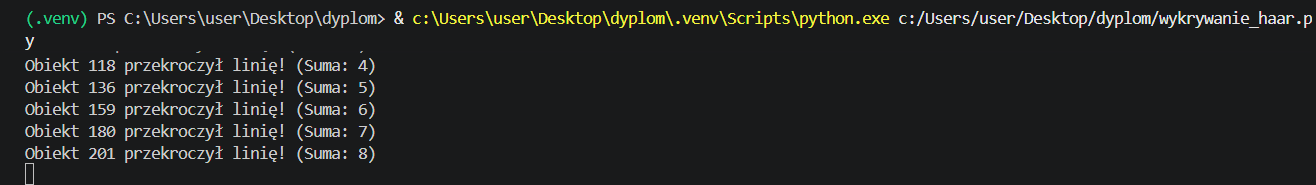
\includegraphics[width=0.95\textwidth]{images/manual4.png}
    \caption{Wydruki w terminalu sygnalizujące przekroczenie linii}
\end{figure}

Identyczny sposób interakcji z użytkownikiem przedstawia wersja programu \textit{wykrywanie\_yolo.py}. Jedyną różnicą pomiędzy programami jest zmiana używanego detektora obiektu z klasyfikatora Haara na sieć YOLO.
Zmiana ta pozwala na poprawienie kilku błędów występujących w pierwotnej wersji tj. niewykrywania części pojazdów, znacznego "pływania" centroidów oraz gubienia detekcji (co po części jest też winą bardzo prostego trackera). Ponadto oba rozwiązania manualne wymagają interakcji z człowiekiem co w przypadku chęci stworzenia dużego systemu obsługującego wiele kamer może być uciążliwe. Z tego względu w dalszych analizach zarzucono przedstawione tutaj rozwiązania i skupiono się bardziej na trybie automatycznym.

Do testów trybu manualnego użyte zostało nagranie pochodzące ze zbioru \href{https://www.kaggle.com/datasets/aryashah2k/highway-traffic-videos-dataset}{Highway Traffic Videos Dataset} o następujących parametrach:
\begin{itemize}
    \item \textbf{rozdzielczość:} 1280x720,
    \item \textbf{liczba klatek na sekundę:} 25,
    \item \textbf{liczba klatek:} 1050,
    \item \textbf{długość:} 42 sekundy,
    \item \textbf{cechy szczególne:} ruch na szerokiej, 3-pasmowej autostradzie, zawiera pojazdy różnego typu - samochody osobowe, busy, ciężarówki, obiekty nagrywane w dosyć pochmurny dzień.
\end{itemize}
\subsection{Tryb automatyczny}
W trybie automatycznym cały proces został podzielony na dwie kluczowe fazy: uczenia oraz roboczą. Na etapie uczenia skrypt \textit{video\_to\_json.py} analizuje za pomocą sieci neuronowej YOLO (wersja YOLO26X) całą sekwencję dostarczoną wsadowo i zapisuje detekcje z każdej klatki do pliku wynikowego w formacie JSON, którego struktura wygląda następująco:
\begin{lstlisting}[language=json]
{
    "track_id": [
        {
            "bbox": [
                ...
            ]
            "confidence": ...,
            "class_name": ...,
            "class_id": 2
        },
        ...
    ],
    ...
}
\end{lstlisting}
Następujące pola zawierają:
\begin{itemize}
    \item \textbf{track\_id} - ID detekcji nadane przez tracker wykorzystywany w sieci YOLO; nawiera on tablicę ze wszystkimi detekcjami danego obiektu z całego nagrania,
    \item \textbf{bbox} - zawiera współrzędne prostokąta otaczającego w formacie XYWH,
    \item \textbf{confidence} - pewność danej detekcji,
    \item \textbf{class\_name} - nazwa klasy według YOLO,
    \item \textbf{class\_id} - ID klasy według sieci YOLO.
\end{itemize}
Mając tak przygotowane dane możemy przejść do następującego etapu fazy uczenia tj. generowania map intensywności obecności obiektów wybranych typów. Zostało to opisane w ramach rozdziału \ref{sec:generowanie}. Natomiast faza robocza zaprezentowana w rozdziale \ref{sec:selekcja}.

W trybie automatycznym zostały wykorzystane nagrania o następujących paramterach:
\begin{table}[H]
\centering
\begin{tabular}{l|c|c|c|c|p{5cm}}
\toprule
     \textbf{Lp.} & \textbf{Rozdzielczość} & \textbf{Liczba FPS} & \textbf{Liczba klatek} & \textbf{Długość} & \textbf{Cechy szczególne}\\
\midrule
    1. & 1920x1080 & 25 & 22500 & 15 minut & dzień, ciekawe sytuacje w ruchu drogowym, skrzyżowanie dwóch dróg \\
    2. & 720x480 & 29.97 & 107805 & 59.95 minut  &  nagranie zaszumione, kamera położona dosyć wysoko, pada deszcz\\
    3. & 720x480 & 29.97 & 107908 & 60.01 minut &  występują tramwaje, zmieniają się warunki atmosferyczne, nagranie nieco zaszumione\\
    4. & 1920x1080 & 25 & 22500 & 15 minut & nagranie o zachodzie słońca, skrzyżowanie dwóch dróg, podobne do nagrania 1 \\
\bottomrule
\end{tabular}
\end{table}
Pochodzą one ze zbioru nagrań z różnych warszawskich ulic, który dostałem od prowadzącego. Na każdym z tych nagrań występują różne kategorie pojazdów takie jak np. autobusy, busy, samochody osobowe, ciężarówki.
\section{Generowanie map intensywności obecności obiektów wybranych typów}
\label{sec:generowanie}
Niniejsza część projektu zrealizowana została w notatniku \textit{aktywacja\_tracking.ipynb}. Na początku wczytujemy uzyskany wcześniej plik JSON z detekcjami do dataframe z pakietu Pandas. Następnie obliczamy przesunięcia obiektów pomiędzy kolejnymi klatkami według następującego algorytmu:
\begin{itemize}
    \item dla pierwszych 30 detekcji danego obiektu przesunięcie wynosi 0,
    \item każde następne przesunięcie obliczane jest ze wzoru\\ $d=\sqrt{(x_{aktualne} - x_{30klatekwczesniej})^2 + (y_{aktualne} - y_{30klatekwczesniej})^2}$.
\end{itemize}
Następnie dla każdej klasy ustalane są minimalne progi przesunięcia pozwalające zaklasyfikować ją do grupy obiektów poruszających się bądź też nieporuszających się. W ramach analizy nagrania dla klas określających pojazdy (car, bus, truch, motorcycle) próg ten wynosi 50.0, a dla klas określających osoby (person, umbrella) próg wynosi 10.0. Na tej podstawie dalej przeprowadzana jest selekcja obiektów do obu grup.

Mając podzielone dane na obiekty poruszające się i nieporuszające możemy przystąpić do generowania właściwych map ciepła. Etap ten zaczyna się od generowania macierzy o rozmiarach równych rozmiarowi klatki obrazu wejściowego. Następnie iterując po każdej detekcji w poszczególnej grupie dodajemy liczbę 1.0 w punkcie w którym występuje centorid detekcji oraz 0.4 w pozostałych punktach należących do ramki otaczającej obiekt. Wprowadzono również dodatkową weryfikację czy współrzędne danej ramki znajdują się w odległości 10 pikseli od krawędzi klatki tak aby uniknąć akumulowania się detekcji na krawędziach spowodowanej perspektywą związaną z oddalaniem się od kamery. Tak wygenerowana macierz jest jeszcze przepuszczana przez filtr Gaussa (z promieniem rozmycia sigma równym 40) tak, aby rozmyć uzyskane w niej wartości. Na podstawie takiej macierzy wygenerowano dalej mapy ciepła.
\subsection{Mapy ciepła dla nagrania nr 1}
\begin{figure}[H]
    \centering
    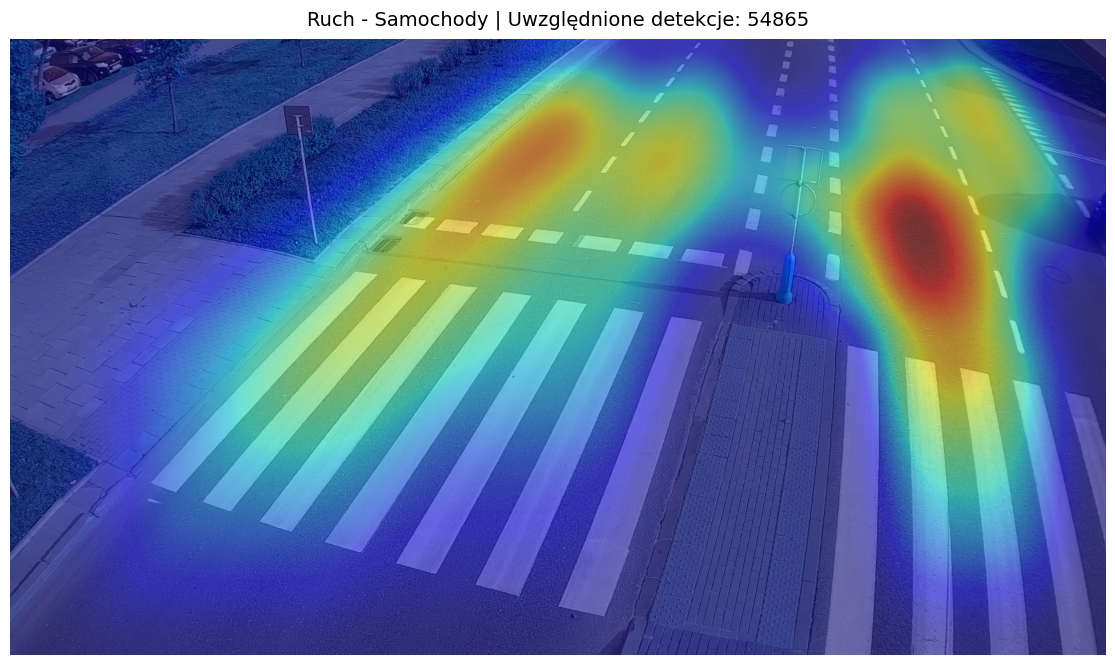
\includegraphics[width=0.90\textwidth]{images/film1/mapa1.png}
    \vfill
    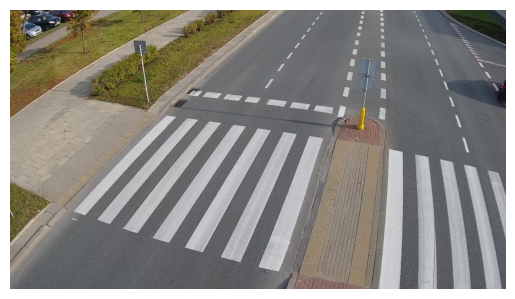
\includegraphics[width=0.90\textwidth]{images/film1/podglad1.png}
    \caption{Mapa ciepła dla obiektów klasy YOLO car, które się poruszają; na dole pierwsza klatka nagrania}
    \label{fig:placeholder}
\end{figure}
\begin{figure}[H]
    \centering
    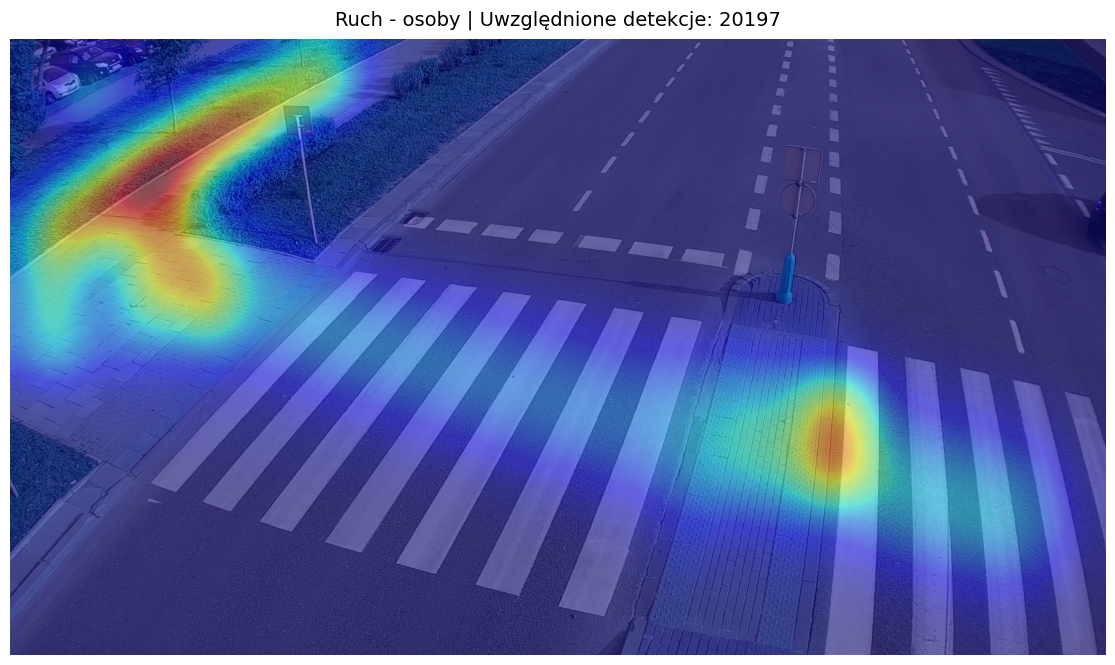
\includegraphics[width=0.90\textwidth]{images/film1/mapa2.png}
    \vfill
    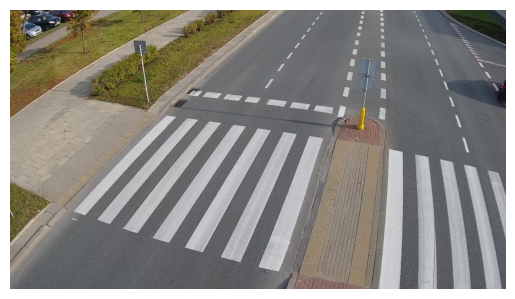
\includegraphics[width=0.90\textwidth]{images/film1/podglad1.png}
    \caption{Mapa ciepła dla obiektów klasy YOLO person, które się poruszają; na dole pierwsza klatka nagrania}
\end{figure}
\begin{figure}[H]
    \centering
    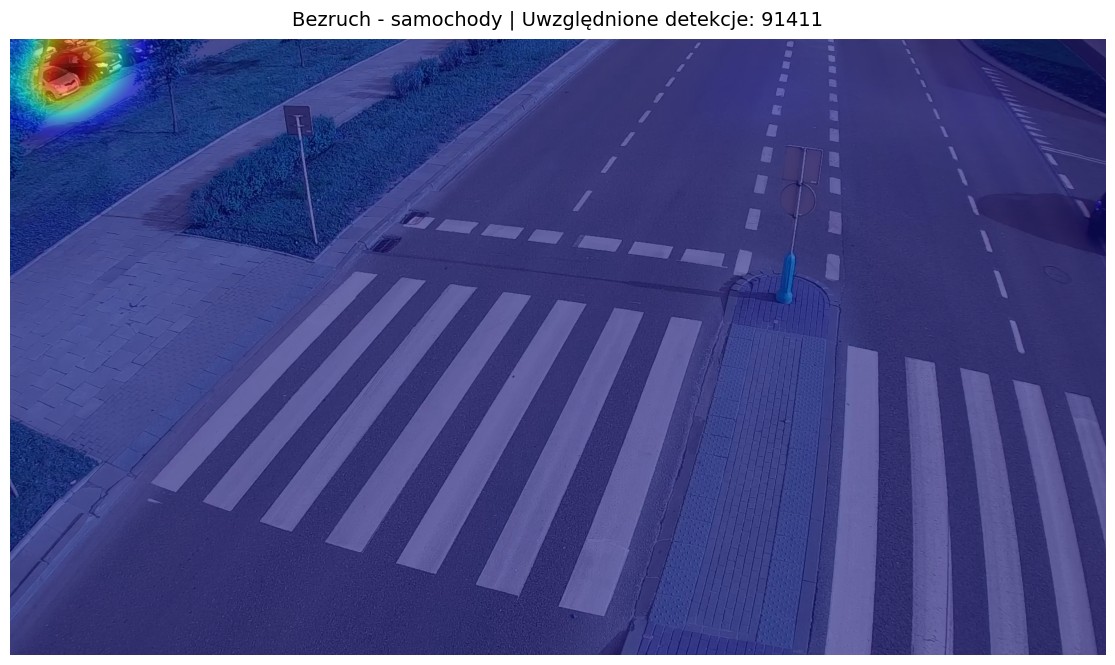
\includegraphics[width=0.90\textwidth]{images/film1/mapa3.png}
    \vfill
    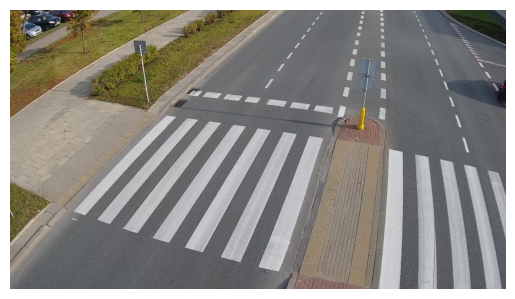
\includegraphics[width=0.90\textwidth]{images/film1/podglad1.png}
    \caption{Mapa ciepła dla obiektów klasy YOLO car, które się nie poruszają; na dole pierwsza klatka nagrania}
\end{figure}
\begin{figure}[H]
    \centering
    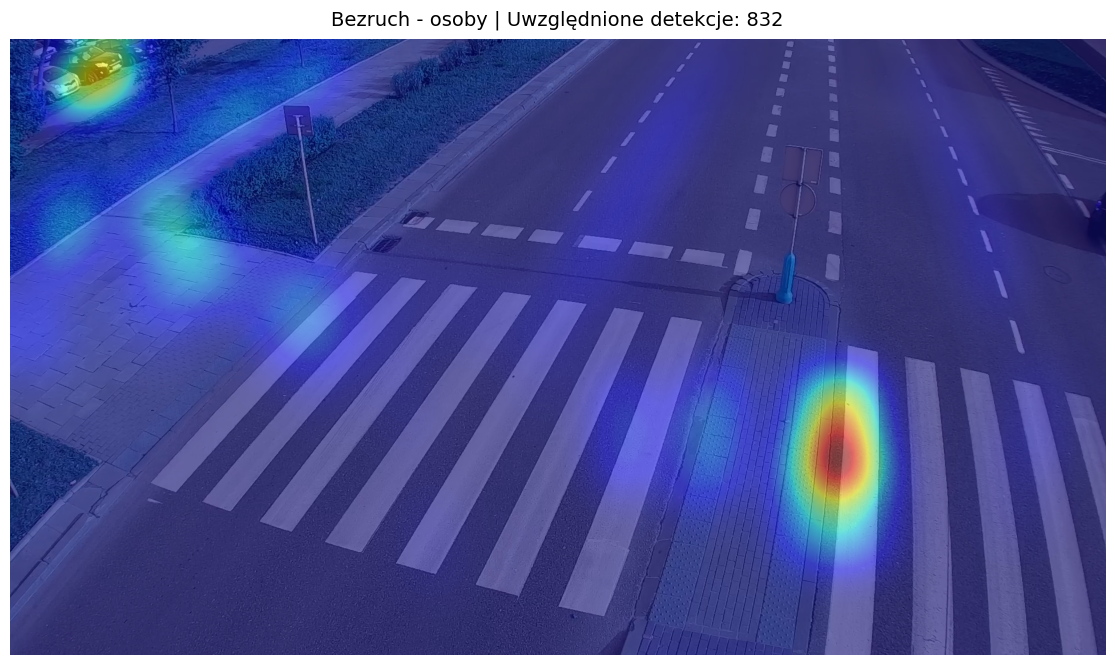
\includegraphics[width=0.90\textwidth]{images/film1/mapa4.png}
    \vfill
    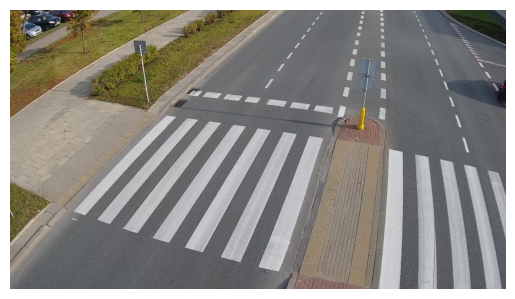
\includegraphics[width=0.90\textwidth]{images/film1/podglad1.png}
    \caption{Mapa ciepła dla obiektów klasy YOLO person, które się nie poruszają; na dole pierwsza klatka nagrania}
\end{figure}
Na wcześniejszych mapach uwzględniono tylko dwie klasy: car i person. Poniżej dokonano jeszcze przypisania obiektów innych klas do dwóch zbiorczych: pojazdy (car, motorcycle, truck, bus) oraz osoby (person, umbrella) i wygenerowano mapy:
\begin{figure}[H]
    \centering
    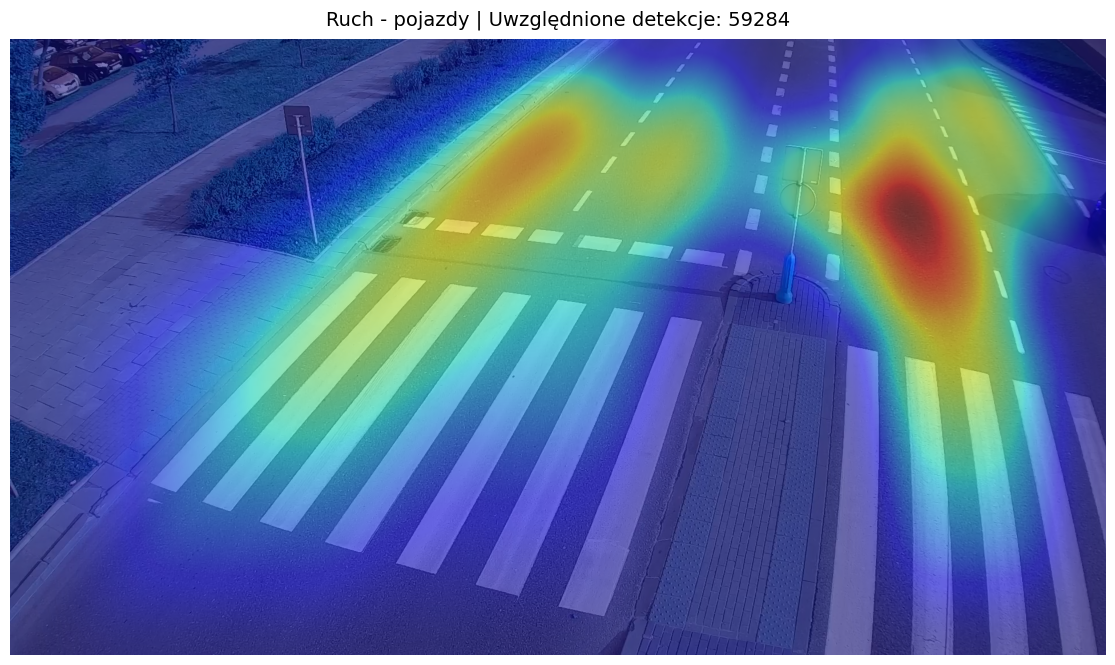
\includegraphics[width=0.90\textwidth]{images/film1/mapa5.png}
    \vfill
    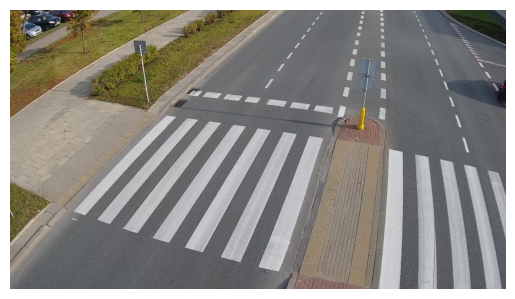
\includegraphics[width=0.90\textwidth]{images/film1/podglad1.png}
    \caption{Mapa ciepła dla zgrupowanych obiektów klasy pojazdy, które się poruszają; na dole pierwsza klatka nagrania}
\end{figure}
\begin{figure}[H]
    \centering
    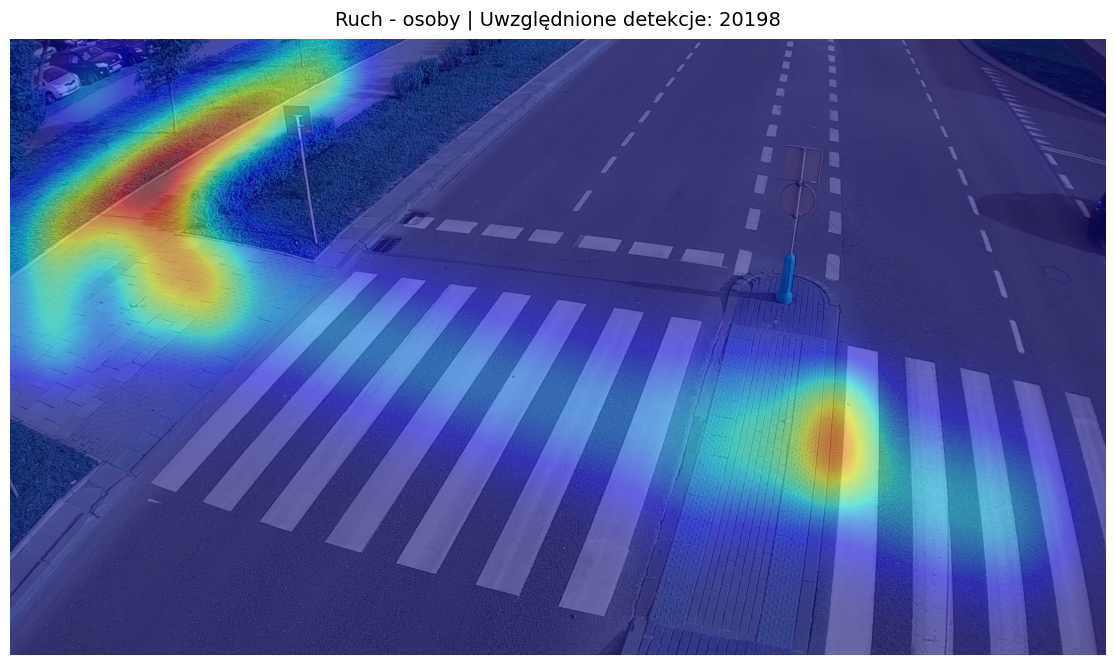
\includegraphics[width=0.90\textwidth]{images/film1/mapa6.png}
    \vfill
    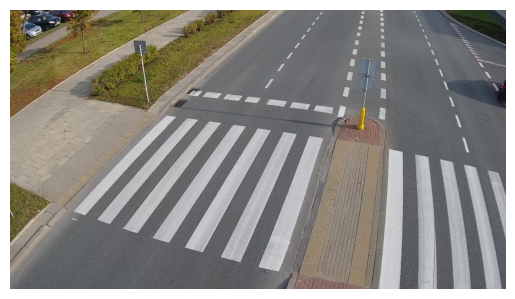
\includegraphics[width=0.90\textwidth]{images/film1/podglad1.png}
    \caption{Mapa ciepła dla  zgrupowanych obiektów klasy osoby, które się poruszają; na dole pierwsza klatka nagrania}
\end{figure}
\textbf{Krótka interpretacja powyższych map:} przygotowany notatnik dosyć dobrze rozróżnia tory ruchu obiektów obu klas dla tego nagrania. Dobrze na wizualizacjach widać miejsca, gdzie samochody parkują, a gdzie poruszają się. Jednakże wzięcie pod uwagę średniego przemieszczenia ma wadę widoczną na mapach - jeśli dany pojazd albo pieszy na chwile się zatrzyma to ta klatka w której się zatrzymał nadal jest brana pod uwagę do grupy obiektów poruszających ze względu na branie pod uwagę średniej. Najbardziej efekt ten widoczny jest w przypadku pieszych, gdzie na krawędzi wyspy oddzielającej pasy ruchu obserwujemy wzrost liczby obserwacji.
\subsection{Mapy ciepła dla nagrania nr 2}
\begin{figure}[H]
    \centering
    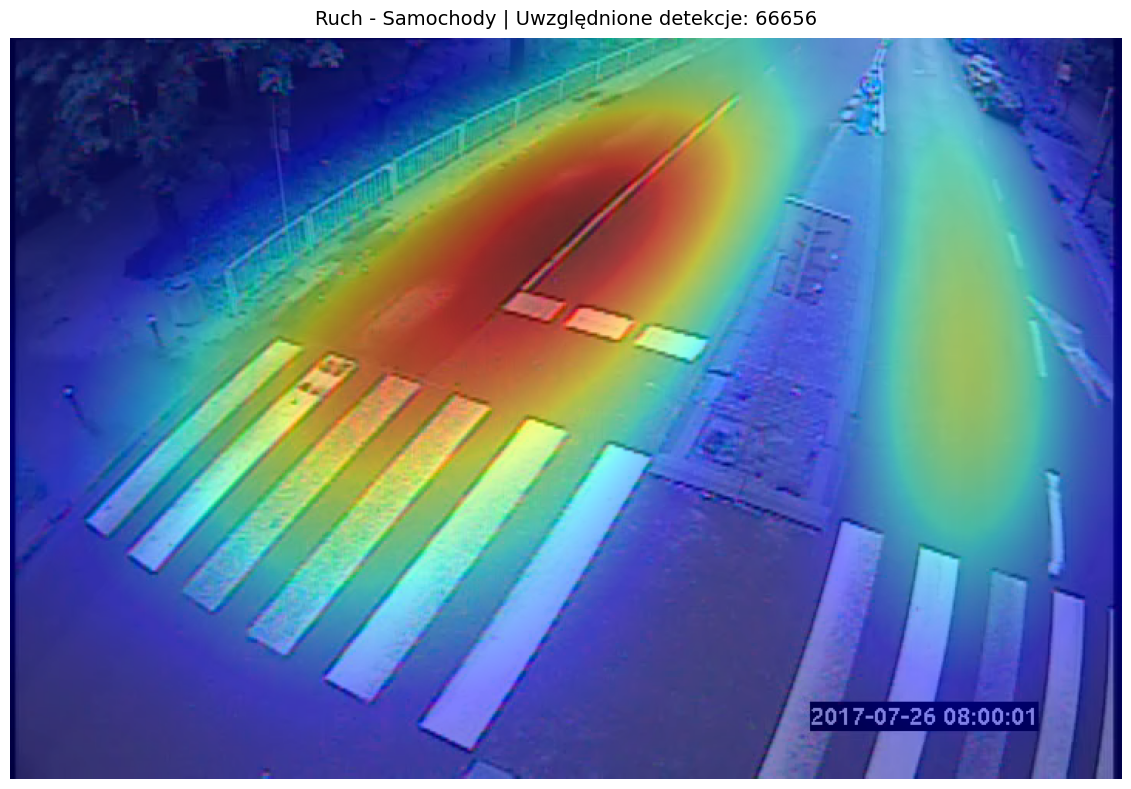
\includegraphics[width=0.90\textwidth]{images/film2/mapa1.png}
    \vfill
    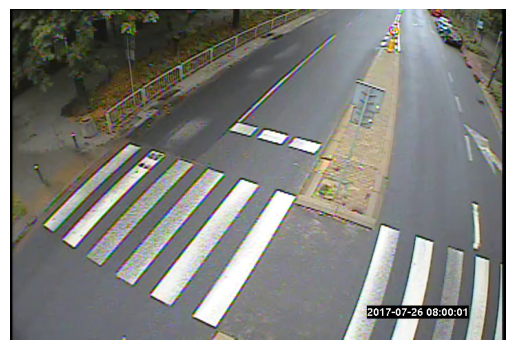
\includegraphics[width=0.90\textwidth]{images/film2/podglad2.png}
    \caption{Mapa ciepła dla obiektów klasy YOLO car, które się poruszają; na dole pierwsza klatka nagrania}
    \label{fig:placeholder}
\end{figure}
\begin{figure}[H]
    \centering
    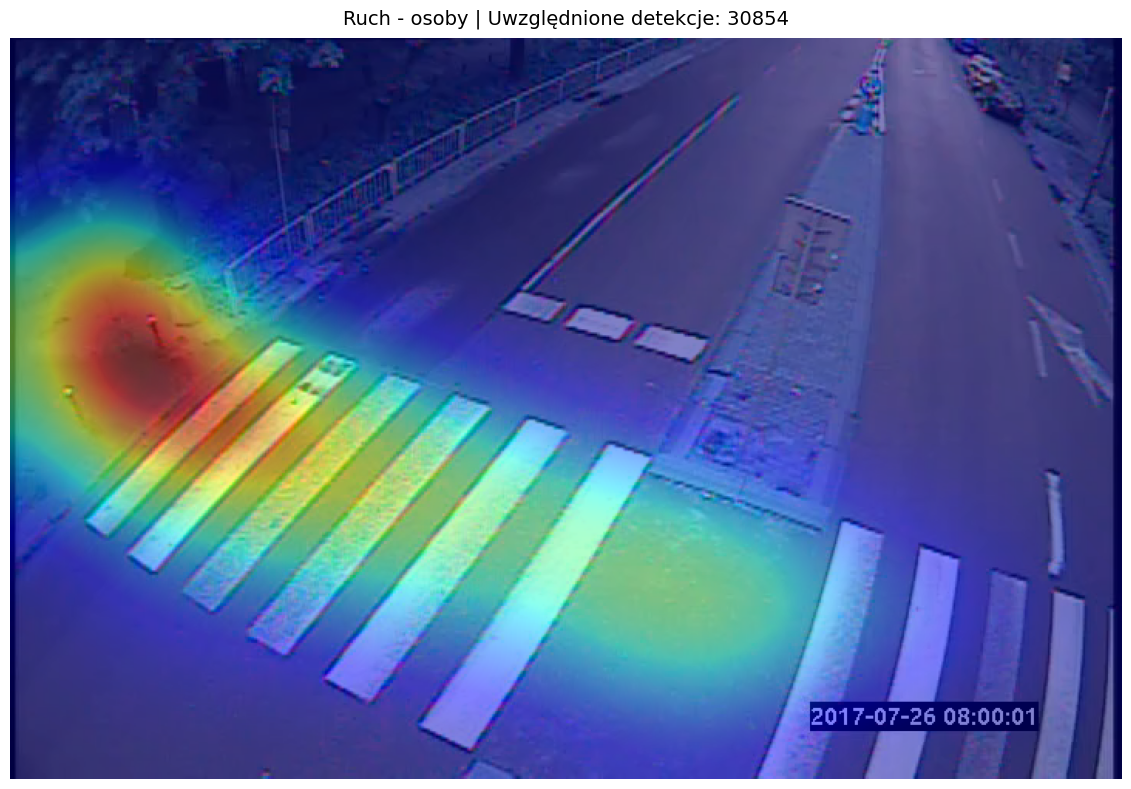
\includegraphics[width=0.90\textwidth]{images/film2/mapa2.png}
    \vfill
    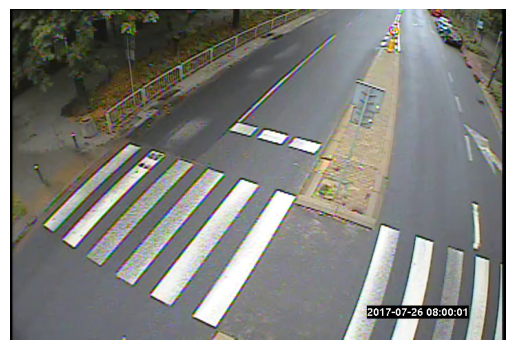
\includegraphics[width=0.90\textwidth]{images/film2/podglad2.png}
    \caption{Mapa ciepła dla obiektów klasy YOLO person, które się poruszają; na dole pierwsza klatka nagrania}
\end{figure}
\begin{figure}[H]
    \centering
    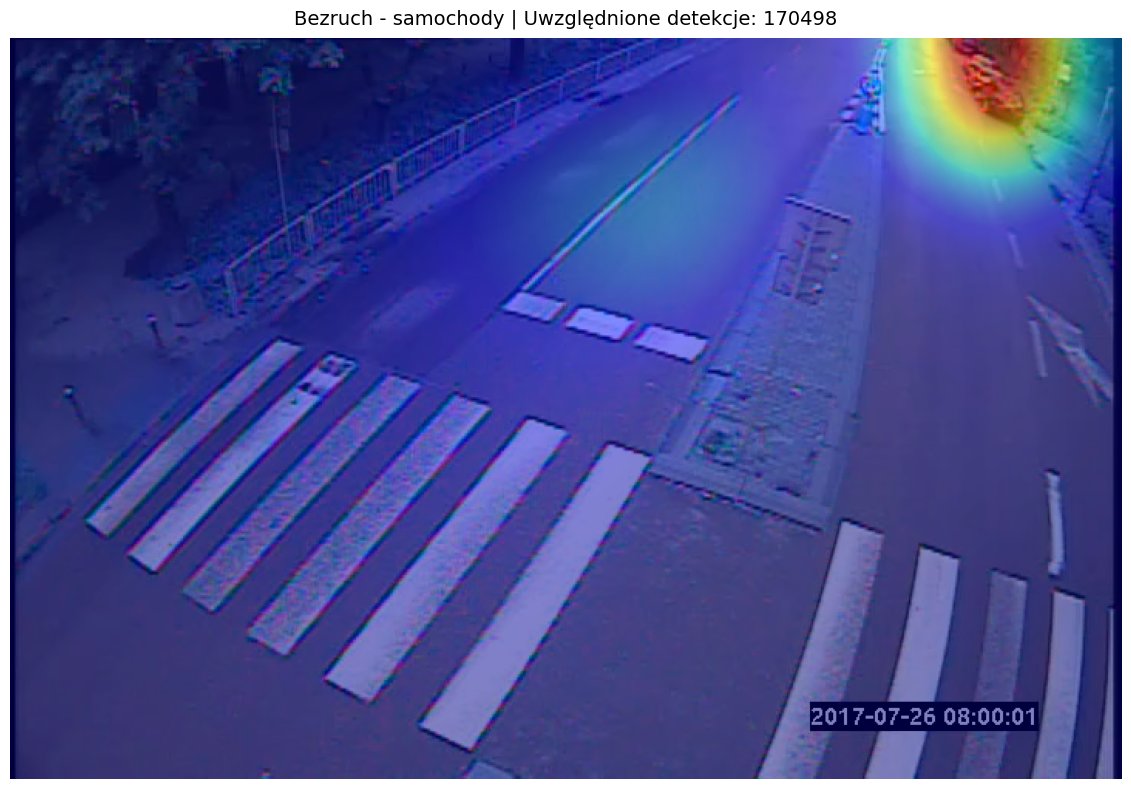
\includegraphics[width=0.90\textwidth]{images/film2/mapa3.png}
    \vfill
    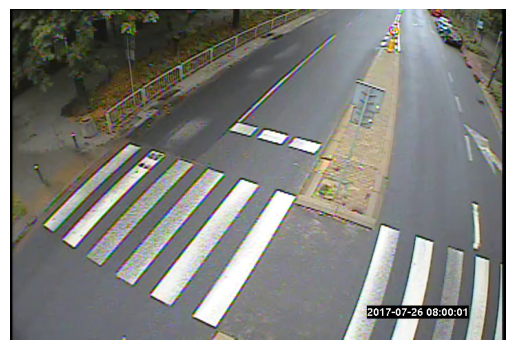
\includegraphics[width=0.90\textwidth]{images/film2/podglad2.png}
    \caption{Mapa ciepła dla obiektów klasy YOLO car, które się nie poruszają; na dole pierwsza klatka nagrania}
\end{figure}
\begin{figure}[H]
    \centering
    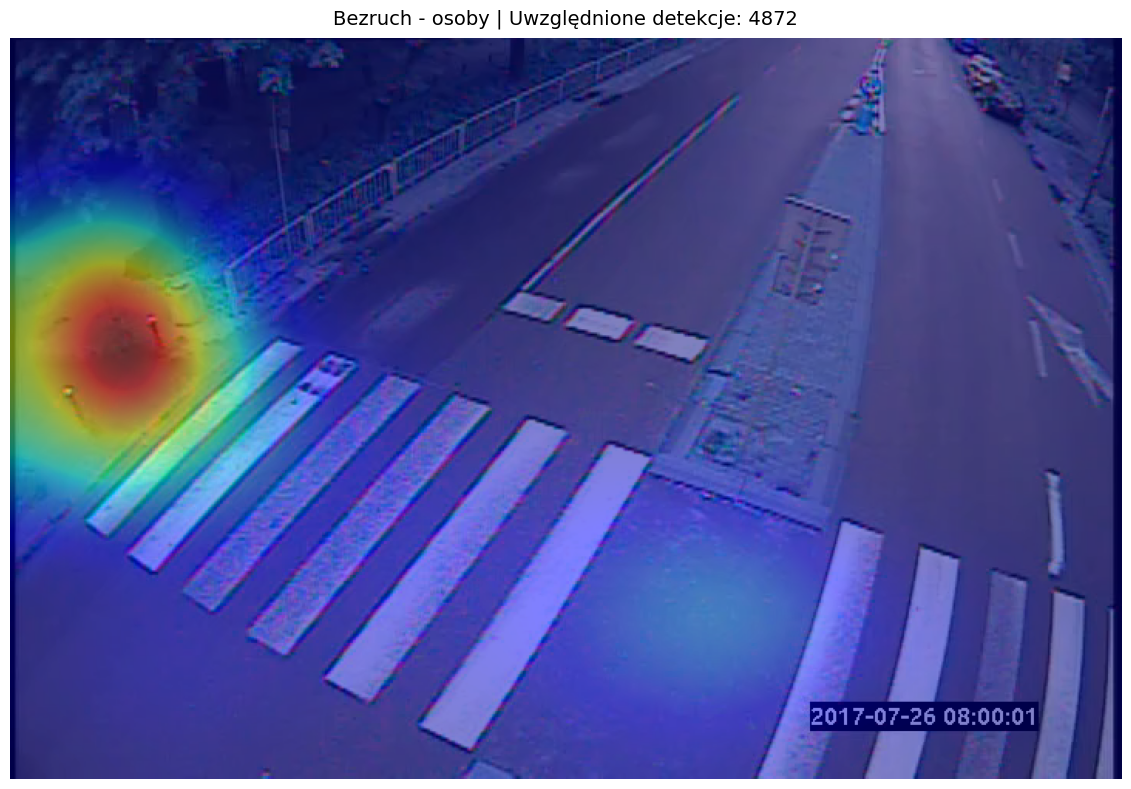
\includegraphics[width=0.90\textwidth]{images/film2/mapa4.png}
    \vfill
    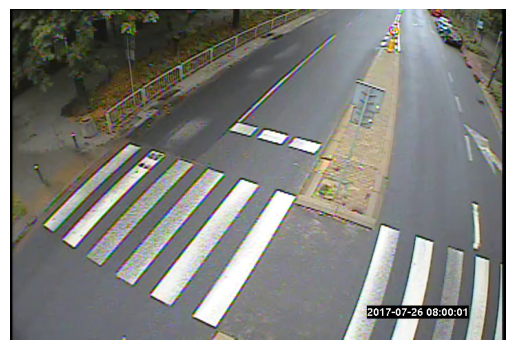
\includegraphics[width=0.90\textwidth]{images/film2/podglad2.png}
    \caption{Mapa ciepła dla obiektów klasy YOLO person, które się nie poruszają; na dole pierwsza klatka nagrania}
\end{figure}
Podobnie jak w przypadku wcześniejszych nagrań wygenerowano również mapy ciepła dla klas zbiorczych:
\begin{figure}[H]
    \centering
    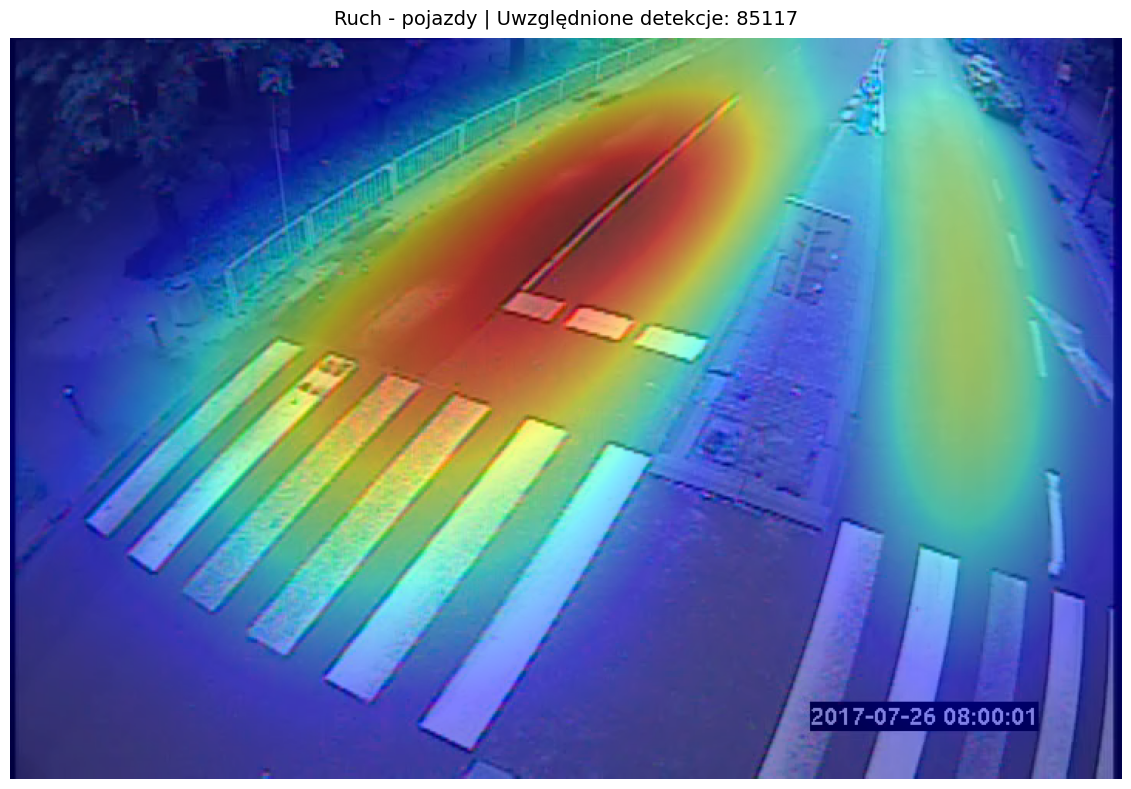
\includegraphics[width=0.90\textwidth]{images/film2/mapa5.png}
    \vfill
    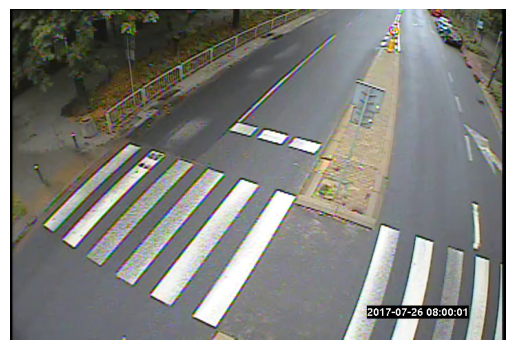
\includegraphics[width=0.90\textwidth]{images/film2/podglad2.png}
    \caption{Mapa ciepła dla zgrupowanych obiektów klasy pojazdy, które się poruszają; na dole pierwsza klatka nagrania}
\end{figure}
\begin{figure}[H]
    \centering
    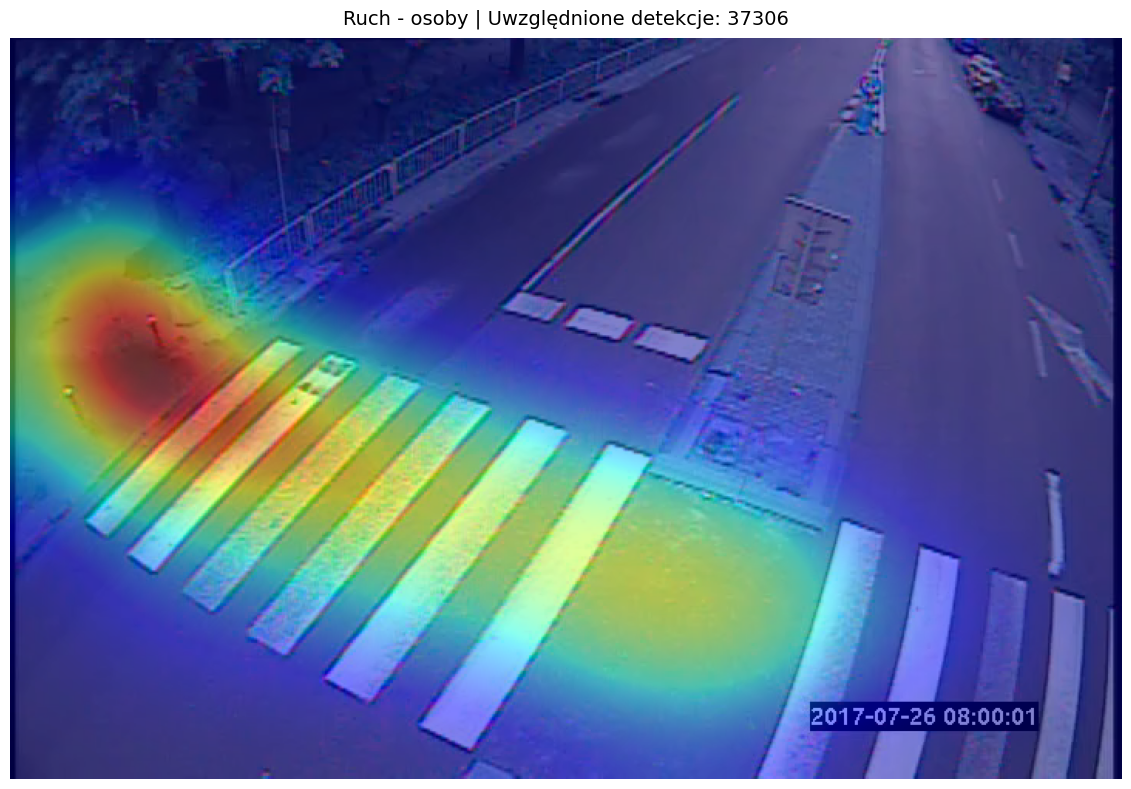
\includegraphics[width=0.90\textwidth]{images/film2/mapa6.png}
    \vfill
    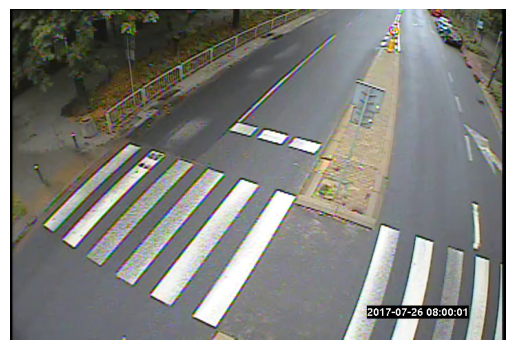
\includegraphics[width=0.90\textwidth]{images/film2/podglad2.png}
    \caption{Mapa ciepła dla  zgrupowanych obiektów klasy osoby, które się poruszają; na dole pierwsza klatka nagrania}
\end{figure}
\textbf{Krótka interpretacja powyższych map:} przygotowany notatnik dosyć dobrze rozróżnia tory ruchu obiektów obu klas dla tego nagrania. Podobnie jak w poprzednim przypadku dobrze widzimy, gdzie np. samochody parkują. Dosyć interesującą jest tutaj na pewno kwestia pieszych w bezruchu przed przejściem dla pieszych. Widzimy, że największa "plama" znajduje się przed wejściem na przejście przez co prawdopodobnie ze względu na omówiony wcześniej mechanizm te detekcje pieszych nawet jeśli zaczną się ruszać nie zostaną zaklasyfikowane do grupy osób poruszających się. Problem ten może obejmować aż ok. 12\% detekcji, dlatego zdecydowanie warto się mu głębiej przyjżeć w przyszłości. Na wizualizacjach możemy również zauważyć pozytywny efekt dodania klasy "umbrella" do kategorii osób. W dzień z którego pochodzi nagranie pada przez co parasolki zasłaniają osoby i zaburzają detekcje. Ponadto kamera jest umieszona dosyć wysoko co powoduje, że widzimy osoby głównie z góry. W ten sposób wykryliśmy dodatkowo ok. 25\% dodatkowych obiektów. Ze względu na napis i margines zapisany w kodzie lewy dolny róg nagrania jest pozbawiony detekcji.
\subsection{Mapy ciepła dla nagrania nr 3}
\begin{figure}[H]
    \centering
    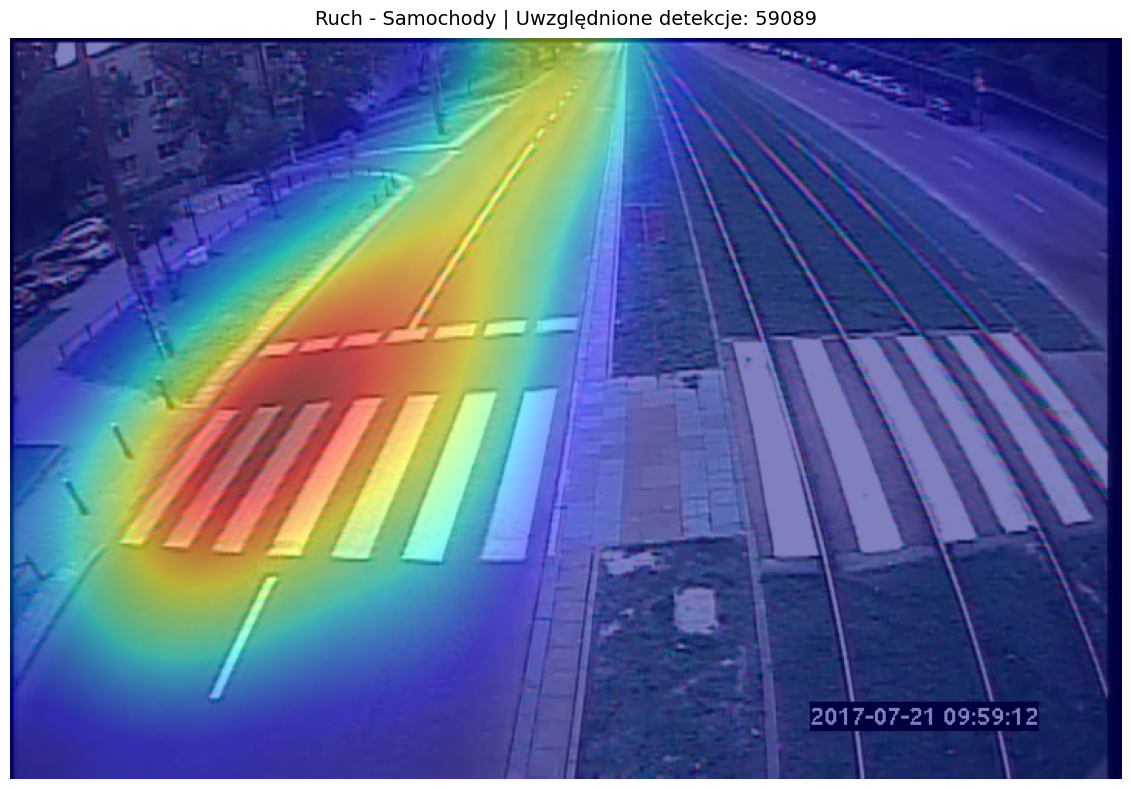
\includegraphics[width=0.90\textwidth]{images/film3/mapa1.png}
    \vfill
    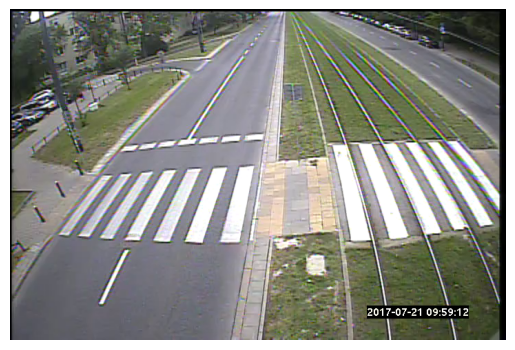
\includegraphics[width=0.90\textwidth]{images/film3/podglad3.png}
    \caption{Mapa ciepła dla obiektów klasy YOLO car, które się poruszają; na dole pierwsza klatka nagrania}
    \label{fig:placeholder}
\end{figure}
\begin{figure}[H]
    \centering
    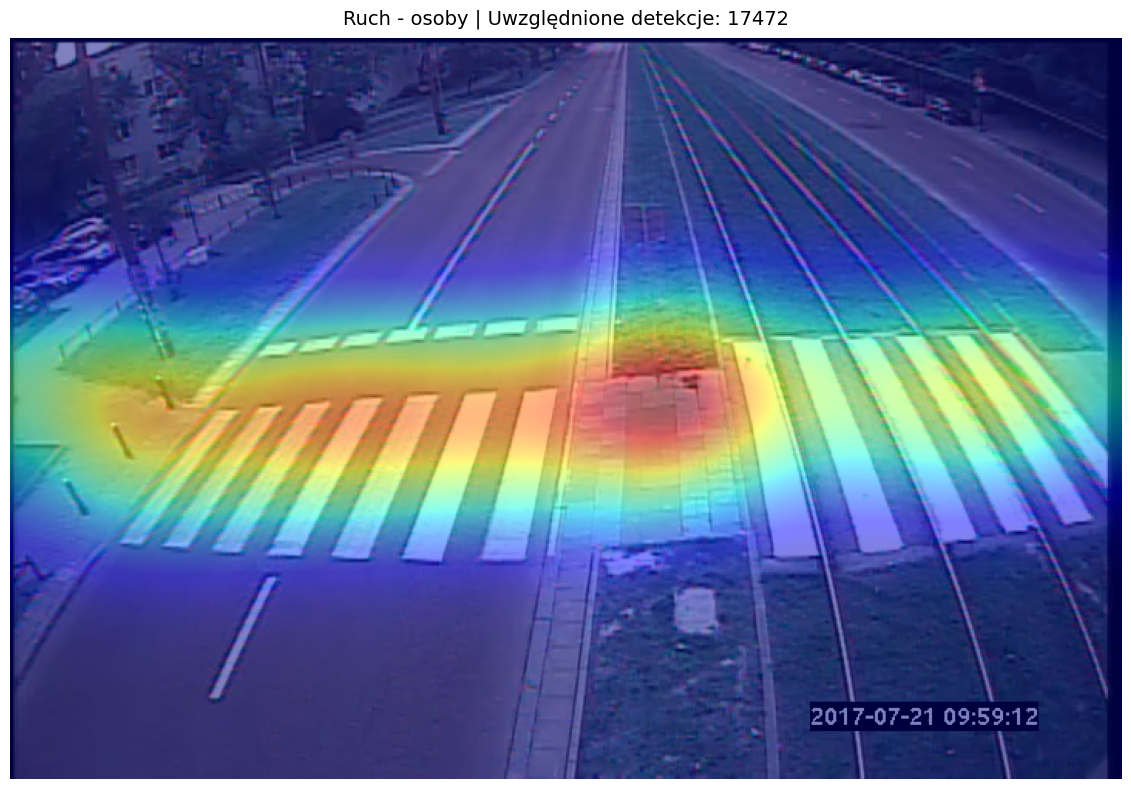
\includegraphics[width=0.90\textwidth]{images/film3/mapa2.png}
    \vfill
    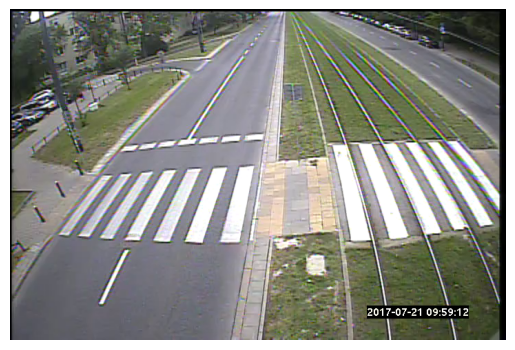
\includegraphics[width=0.90\textwidth]{images/film3/podglad3.png}
    \caption{Mapa ciepła dla obiektów klasy YOLO person, które się poruszają; na dole pierwsza klatka nagrania}
\end{figure}
\begin{figure}[H]
    \centering
    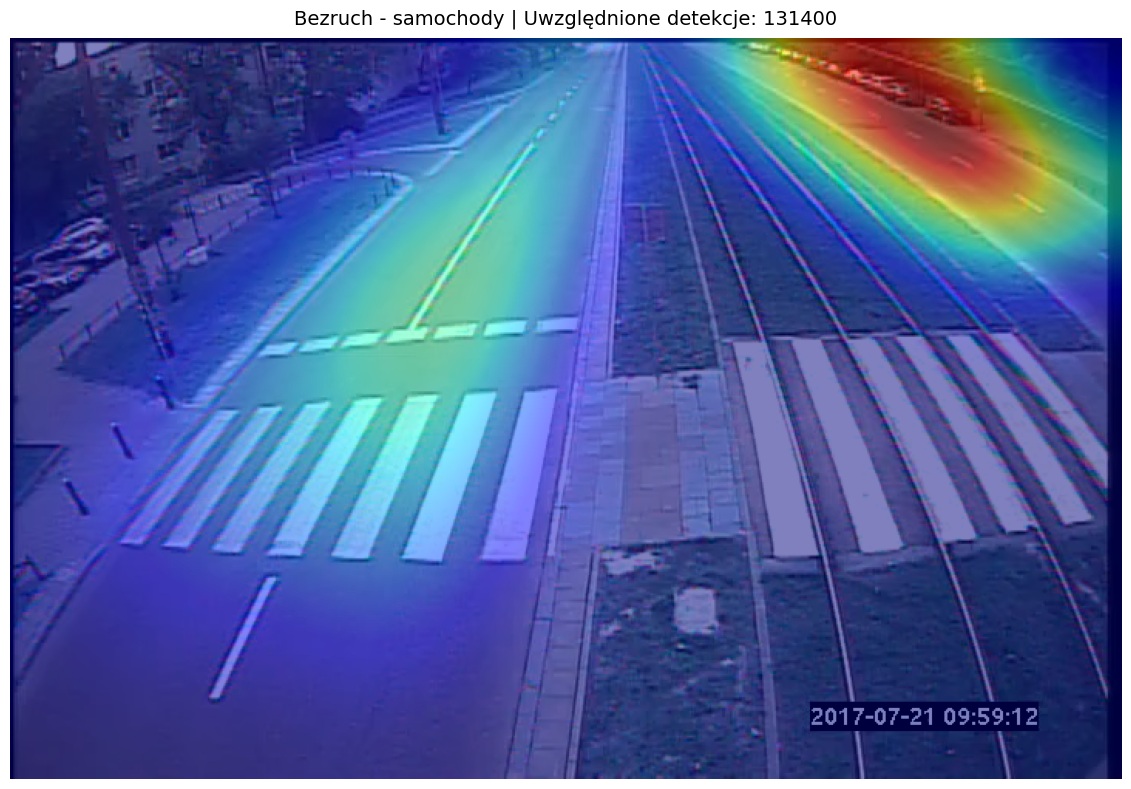
\includegraphics[width=0.90\textwidth]{images/film3/mapa3.png}
    \vfill
    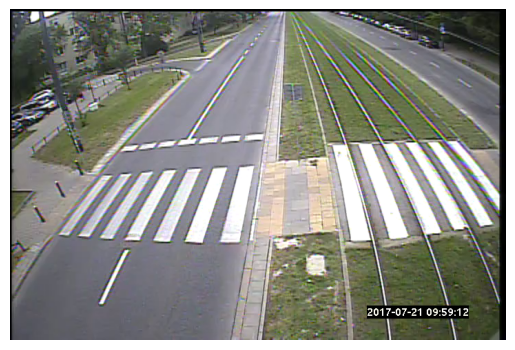
\includegraphics[width=0.90\textwidth]{images/film3/podglad3.png}
    \caption{Mapa ciepła dla obiektów klasy YOLO car, które się nie poruszają; na dole pierwsza klatka nagrania}
\end{figure}
\begin{figure}[H]
    \centering
    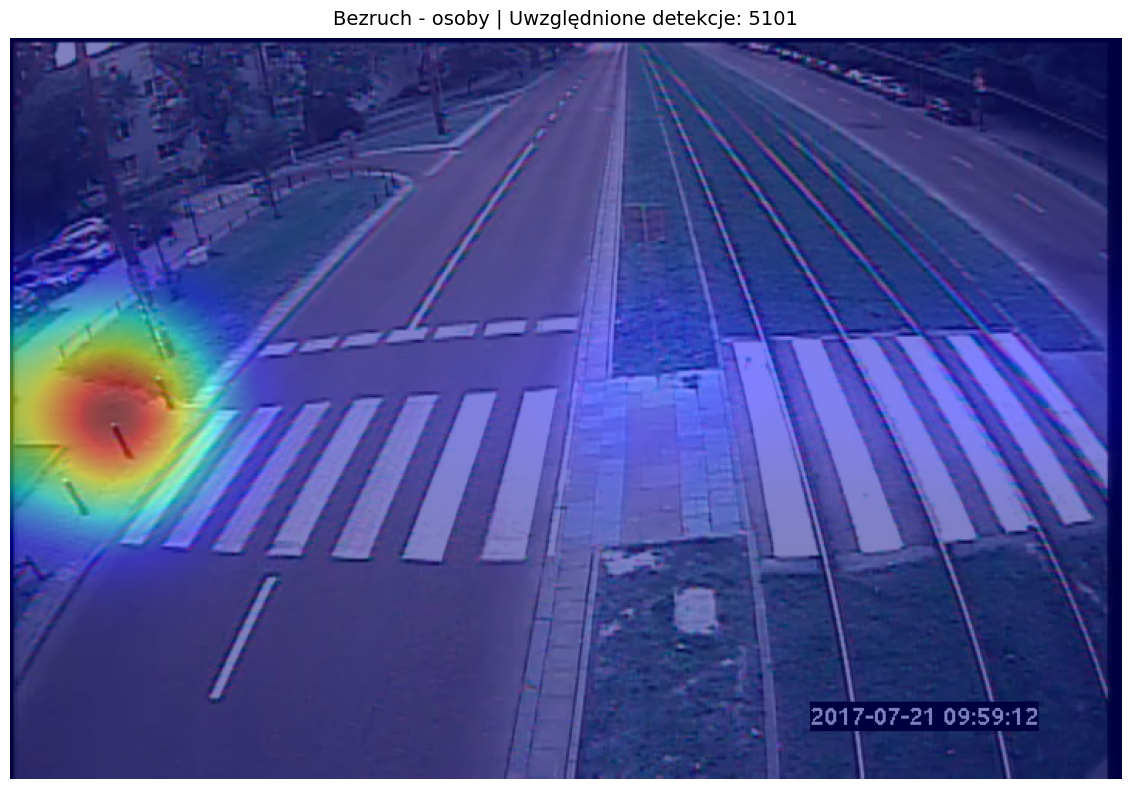
\includegraphics[width=0.90\textwidth]{images/film3/mapa4.png}
    \vfill
    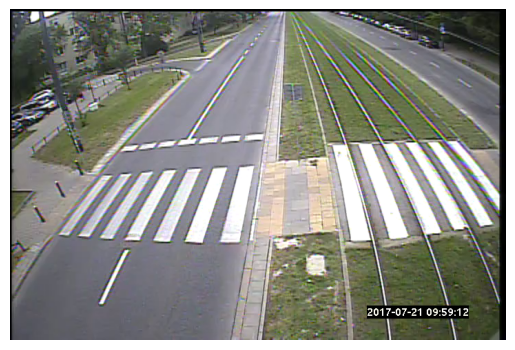
\includegraphics[width=0.90\textwidth]{images/film3/podglad3.png}
    \caption{Mapa ciepła dla obiektów klasy YOLO person, które się nie poruszają; na dole pierwsza klatka nagrania}
\end{figure}
Podobnie jak w przypadku wcześniejszego nagrania wygenerowano również mapy ciepła dla klas zbiorczych:
\begin{figure}[H]
    \centering
    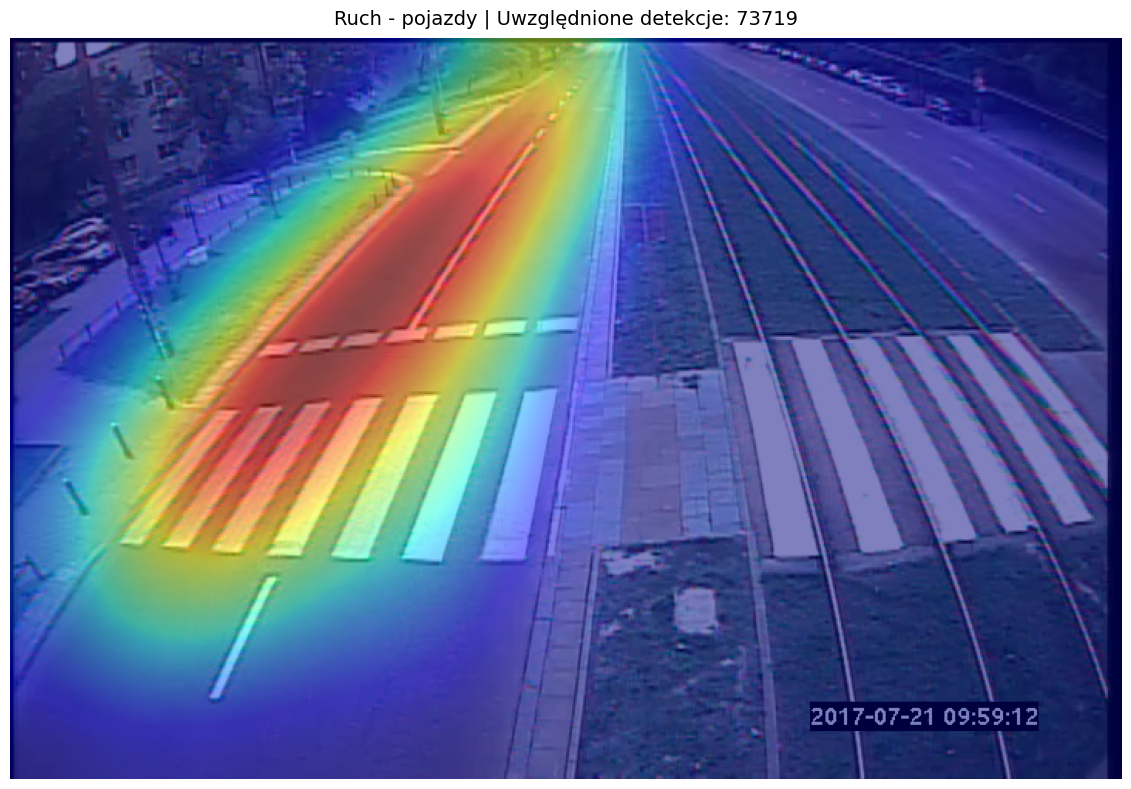
\includegraphics[width=0.90\textwidth]{images/film3/mapa5.png}
    \vfill
    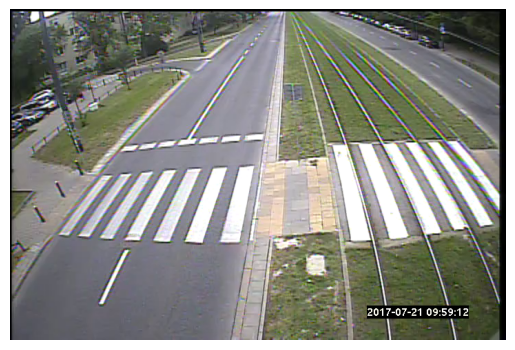
\includegraphics[width=0.90\textwidth]{images/film3/podglad3.png}
    \caption{Mapa ciepła dla zgrupowanych obiektów klasy pojazdy, które się poruszają; na dole pierwsza klatka nagrania}
\end{figure}
\begin{figure}[H]
    \centering
    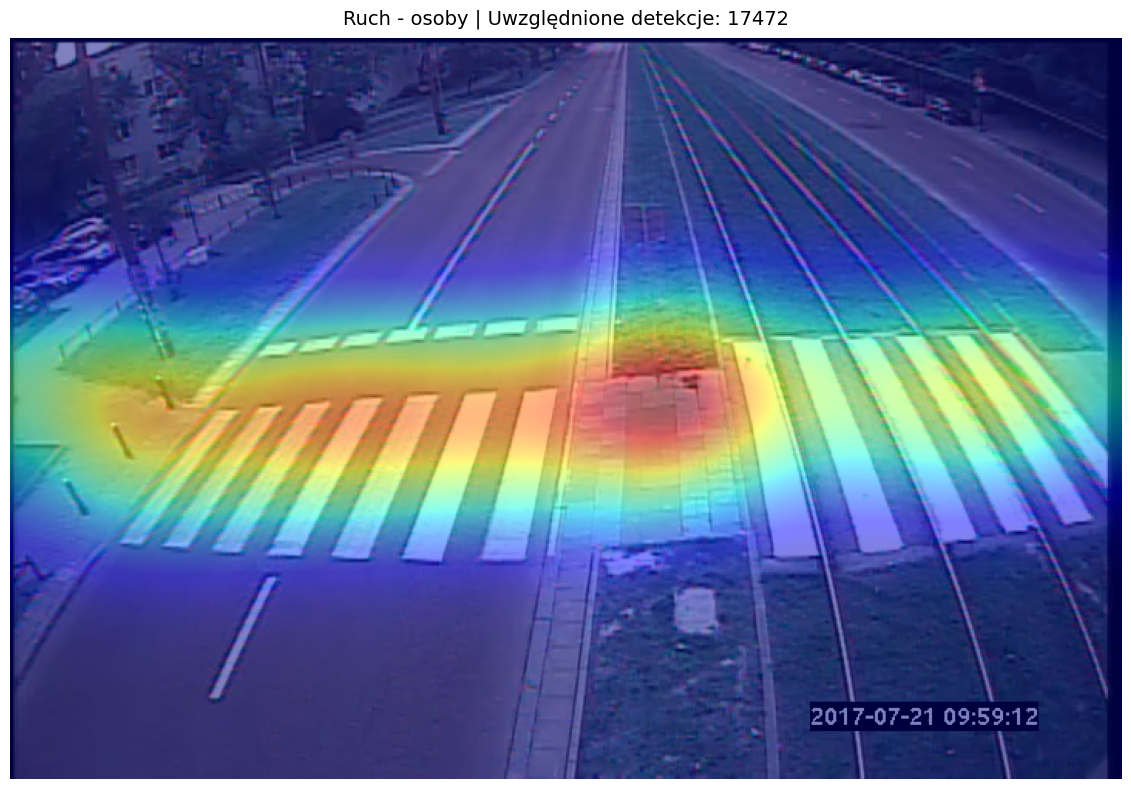
\includegraphics[width=0.90\textwidth]{images/film3/mapa6.png}
    \vfill
    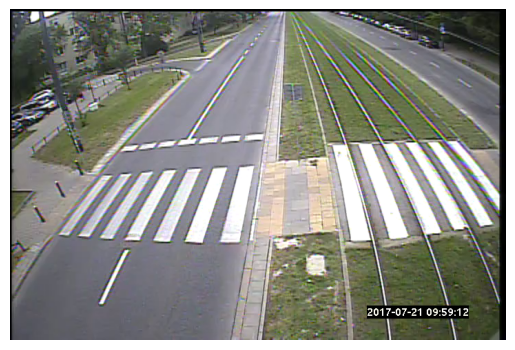
\includegraphics[width=0.90\textwidth]{images/film3/podglad3.png}
    \caption{Mapa ciepła dla  zgrupowanych obiektów klasy osoby, które się poruszają; na dole pierwsza klatka nagrania}
\end{figure}
\textbf{Krótka interpretacja powyższych map:} przygotowany notatnik bardzo dobrze rozróżnia pasy ruchu dla obiektów poszczególnych typów. Prawie cała ulica i przejście dla pieszych pokryte są detekcjami obiektów odpowiadających im typów. Ciekawą kwestią jest na tym nagraniu torowisko tramwajowe. Warto byłoby tutaj rozważyć dodanie dodatkowej grupy reprezentującej pojazdy szynowe do notatnika lub dołączenie pojazdów szynowych do instniejącej już grupy pojazdów. Kawałek drogi widoczny w prawym górnym rogu prawie całkowicie został pokryty pojazdami, które się nie poruszają. Może to być moim zdaniem spowodowane niską rozdzielczością nagrania, lecz nie przeszkadza to w badanym przeze mnie problemie ze względu na brak punktów wspólnych tamtego pasa ruchu z przejściem dla pieszych.
\subsection{Mapy ciepła dla nagrania nr 4}
\begin{figure}[H]
    \centering
    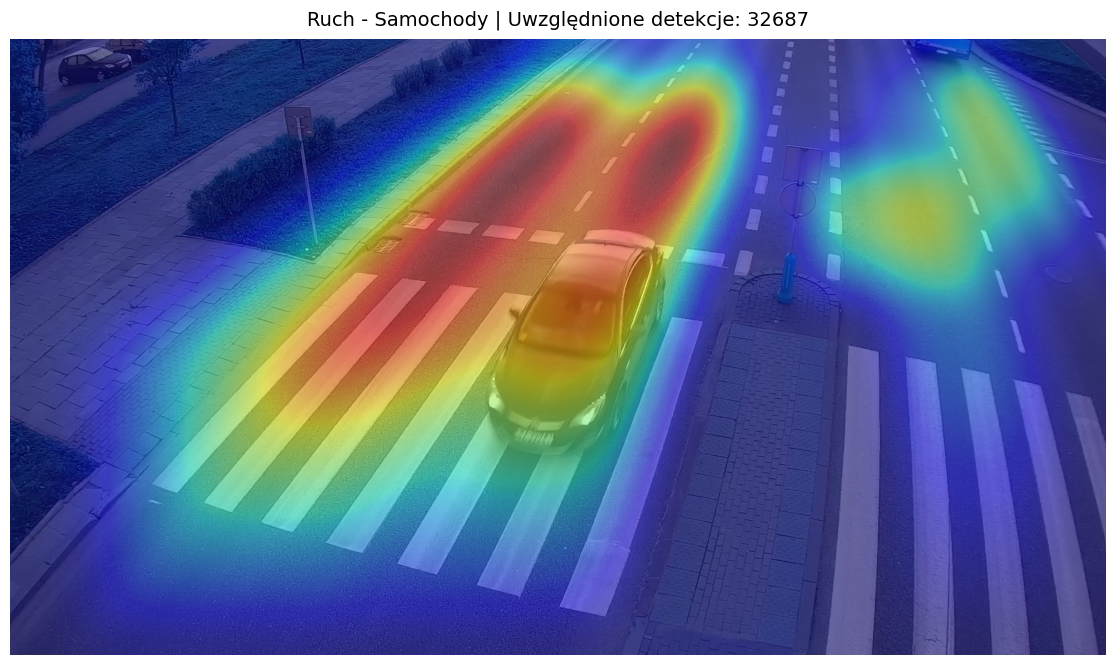
\includegraphics[width=0.90\textwidth]{images/film4/mapa1.png}
    \vfill
    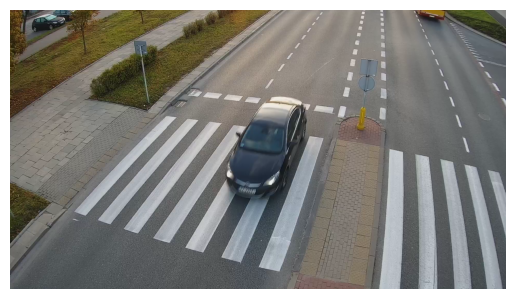
\includegraphics[width=0.90\textwidth]{images/film4/podglad4.png}
    \caption{Mapa ciepła dla obiektów klasy YOLO car, które się poruszają; na dole pierwsza klatka nagrania}
    \label{fig:placeholder}
\end{figure}
\begin{figure}[H]
    \centering
    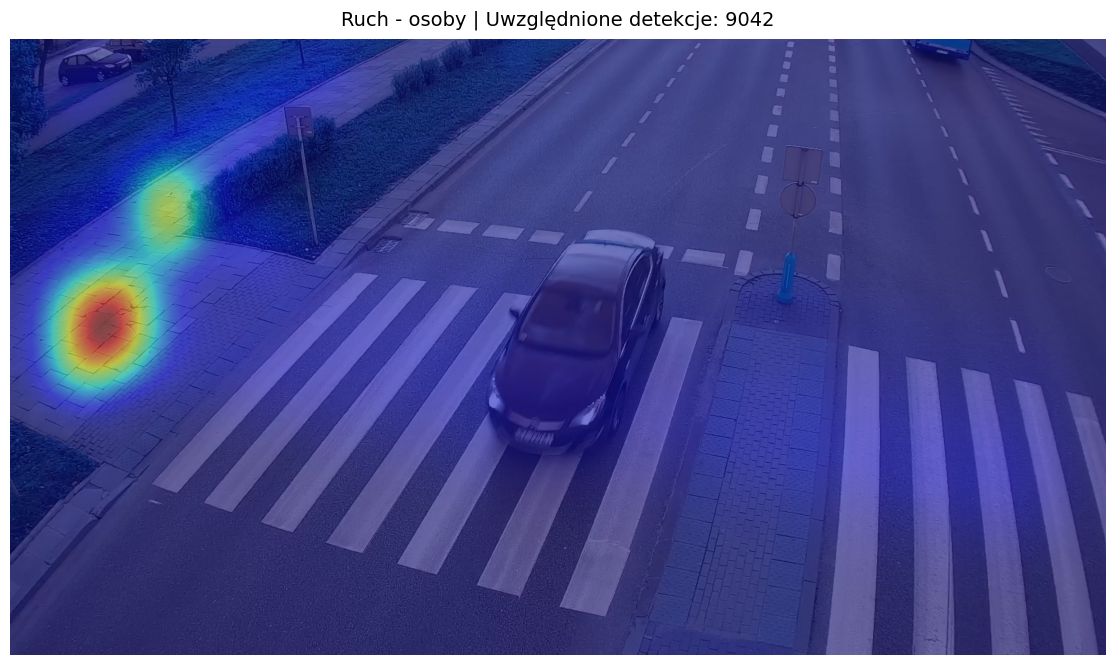
\includegraphics[width=0.90\textwidth]{images/film4/mapa2.png}
    \vfill
    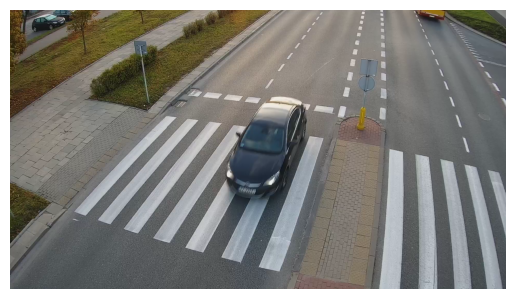
\includegraphics[width=0.90\textwidth]{images/film4/podglad4.png}
    \caption{Mapa ciepła dla obiektów klasy YOLO person, które się poruszają; na dole pierwsza klatka nagrania}
\end{figure}
\begin{figure}[H]
    \centering
    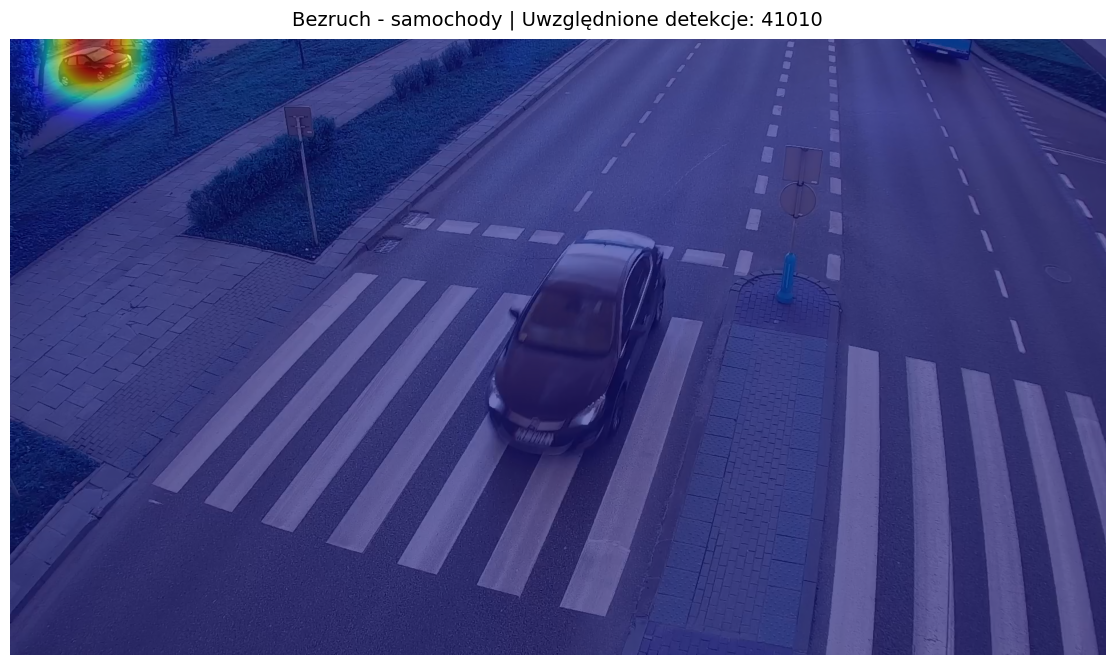
\includegraphics[width=0.90\textwidth]{images/film4/mapa3.png}
    \vfill
    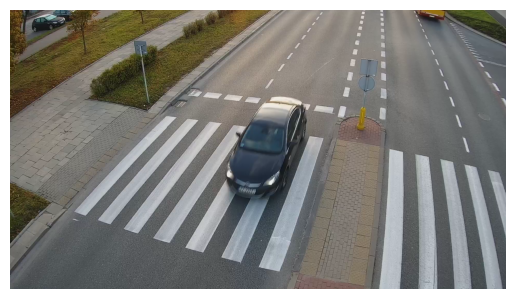
\includegraphics[width=0.90\textwidth]{images/film4/podglad4.png}
    \caption{Mapa ciepła dla obiektów klasy YOLO car, które się nie poruszają; na dole pierwsza klatka nagrania}
\end{figure}
\begin{figure}[H]
    \centering
    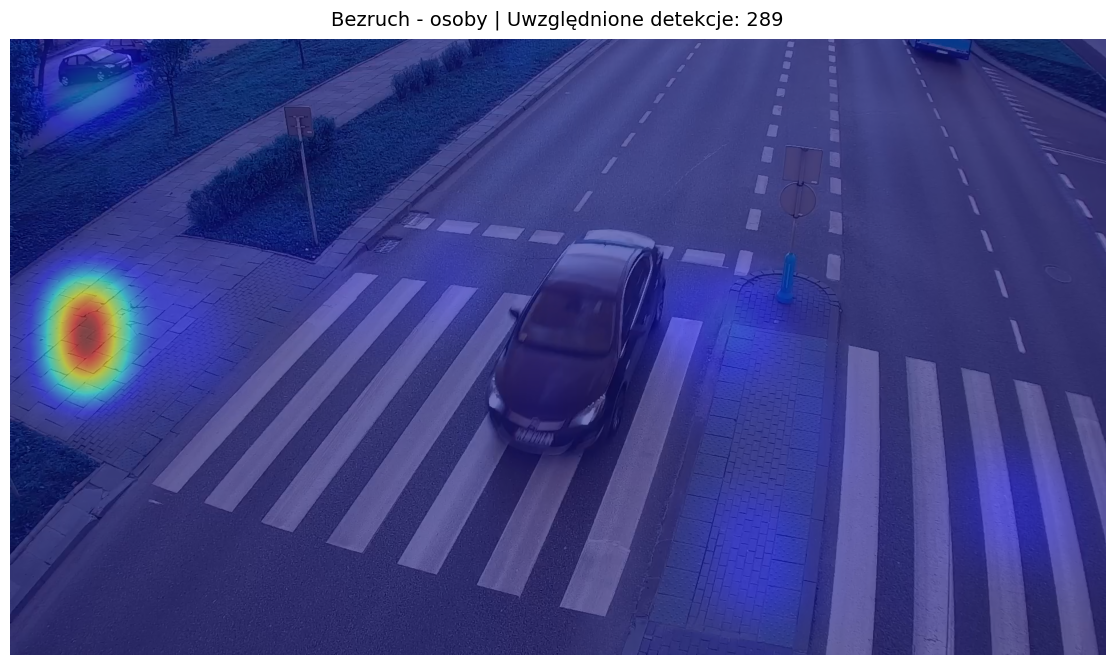
\includegraphics[width=0.90\textwidth]{images/film4/mapa4.png}
    \vfill
    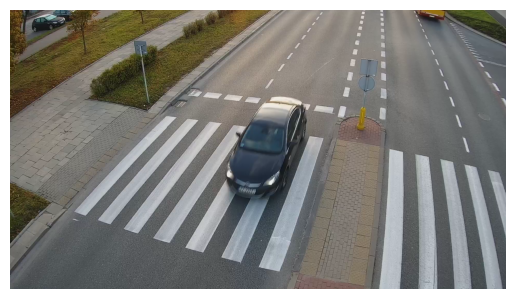
\includegraphics[width=0.90\textwidth]{images/film4/podglad4.png}
    \caption{Mapa ciepła dla obiektów klasy YOLO person, które się nie poruszają; na dole pierwsza klatka nagrania}
\end{figure}
Podobnie jak w przypadku wcześniejszych nagrań wygenerowano również mapy ciepła dla klas zbiorczych:
\begin{figure}[H]
    \centering
    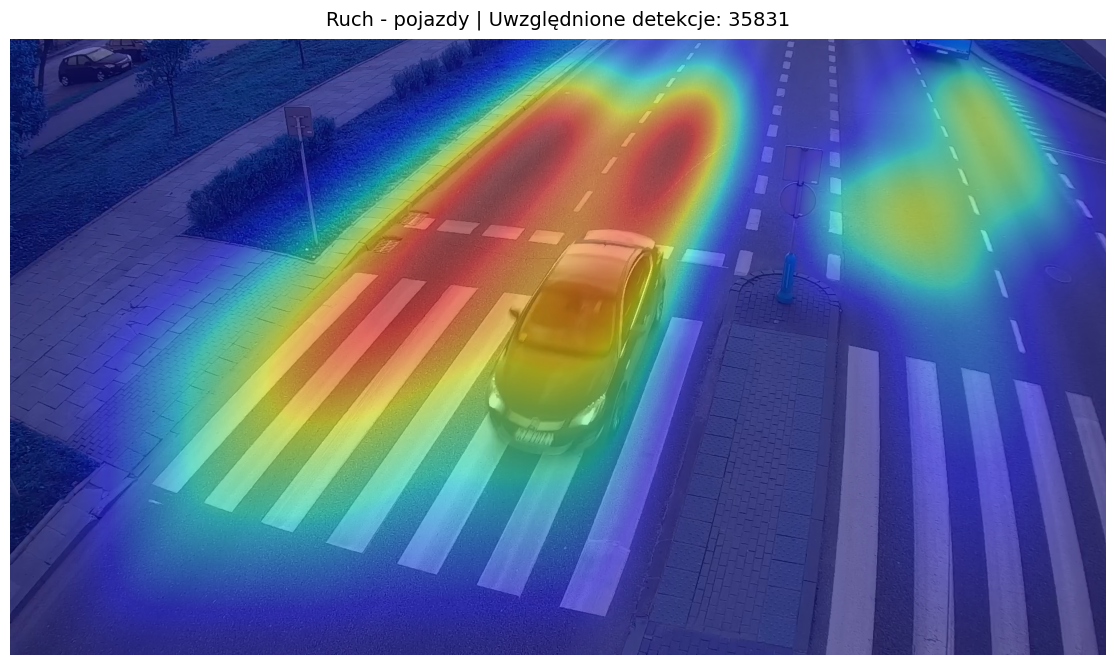
\includegraphics[width=0.90\textwidth]{images/film4/mapa5.png}
    \vfill
    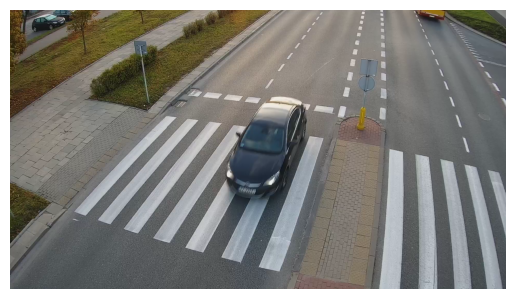
\includegraphics[width=0.90\textwidth]{images/film4/podglad4.png}
    \caption{Mapa ciepła dla zgrupowanych obiektów klasy pojazdy, które się poruszają; na dole pierwsza klatka nagrania}
\end{figure}
\begin{figure}[H]
    \centering
    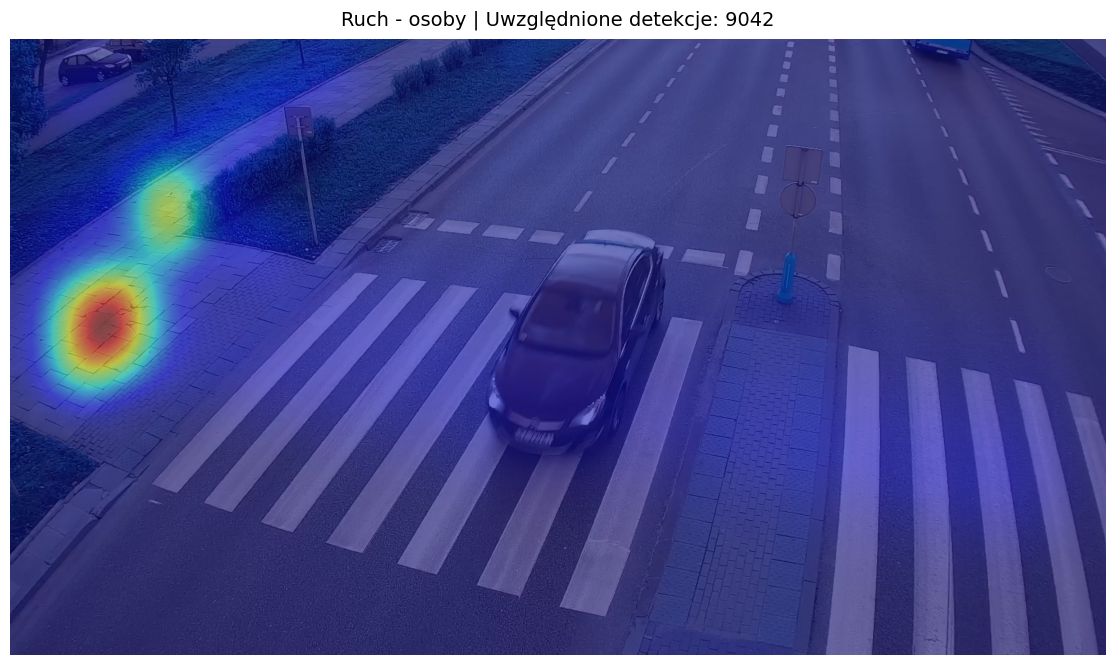
\includegraphics[width=0.90\textwidth]{images/film4/mapa6.png}
    \vfill
    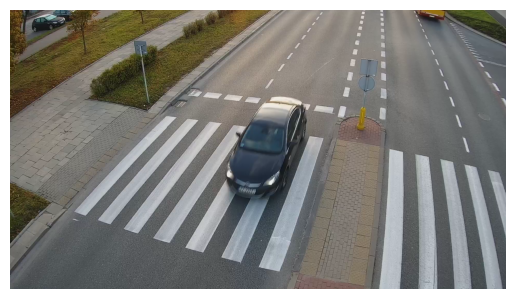
\includegraphics[width=0.90\textwidth]{images/film4/podglad4.png}
    \caption{Mapa ciepła dla  zgrupowanych obiektów klasy osoby, które się poruszają; na dole pierwsza klatka nagrania}
\end{figure}
\textbf{Krótka interpretacja powyższych map:} w tym przypadku uzyskane wyniki możemy porównywać z mapami dla nagrania nr 1. Jest to to same ujęcie, ale w innej chwili. Zdecydowanie poprawiło się wykyrwanie pojazdów w lewej części nagrania, lecz jednocześnie pogroszyło się ono dla prawej części. Również gorzej wypadło wykyrwanie torów ruchu pieszych. Być może jest to kwestia doboru odpowiednich parametrów takich jak progi średniego przemieszczenia. Warto pochylić się nad tą kwestią w przyszłości i zbadać ich wpływ na to nagranie. Być może dzięki tym zmianom bylibyśmy w stanie ograniczyć nagromadzenie detekcji pieszych przed przejściem w kategorii osoby ruch.
\section{Tworzenie pól interakcji obiektów różnych typów}
Przygotowane w rozdziale \ref{sec:generowanie} macierze interakcji dla dwóch głównych klas: pojazdy i osoby pozwalają na wyznaczenie ich pól interakcji. W dalszej części notatnika \textit{aktywacja\_tracking.py} dokonuję to poprzez pomnożenie każdego elementu z pierwszej macierzy z jego odpowiednikiem z drugiej i dokonaniem normalizacji na przedział [0,1]. Dla takiej macierzy również wygenerowane zostały mapy interakcji:
\begin{figure}[H]
    \centering
    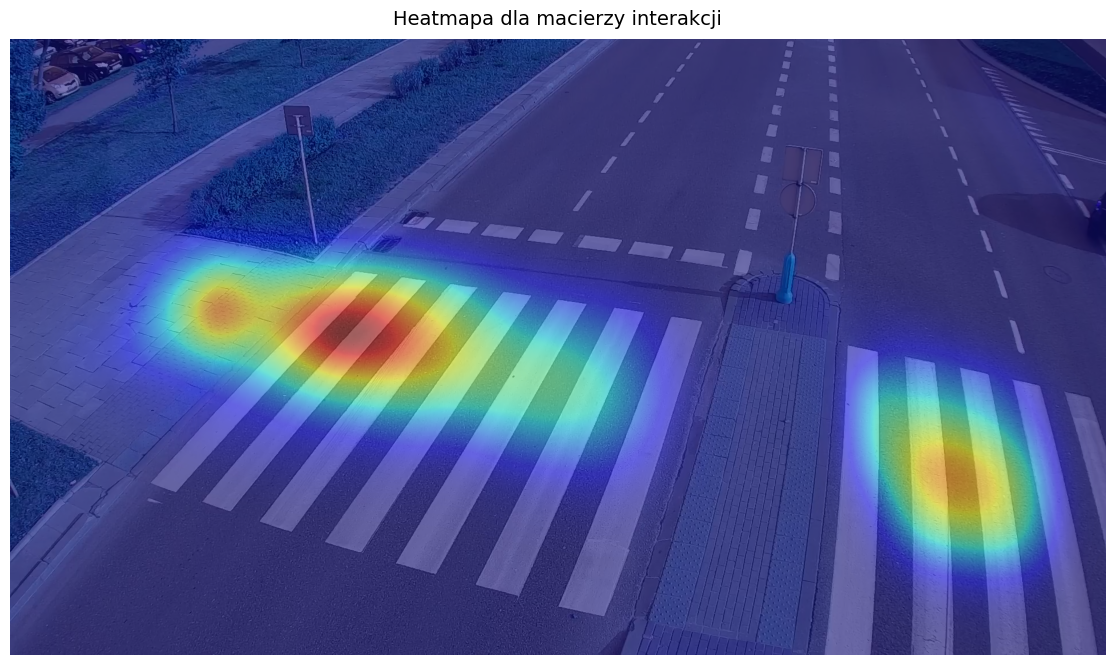
\includegraphics[width=0.95\textwidth]{images/film1/mapa7.png}
    \caption{Mapa ciepła wygenerowana dla macierzy interakcji pomiędzy obiektami klasy pojazdy i osoby dla nagrania nr 1}
\end{figure}
\begin{figure}[H]
    \centering
    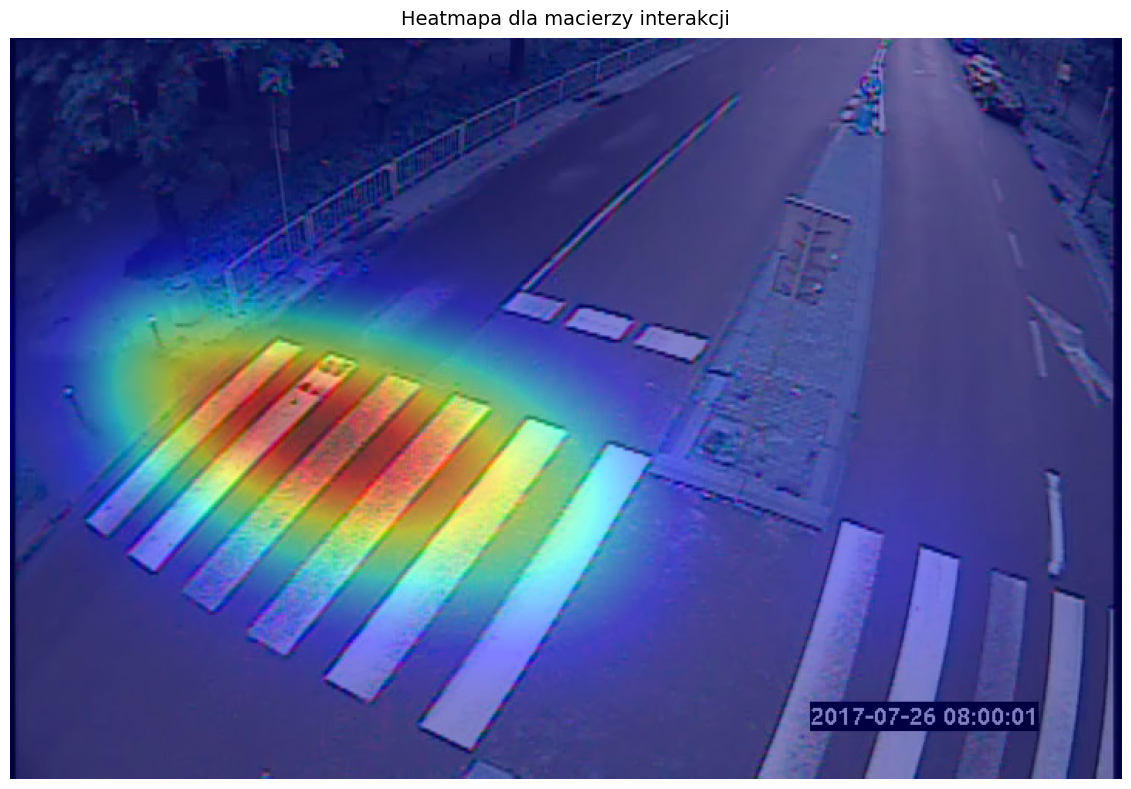
\includegraphics[width=0.95\textwidth]{images/film2/mapa7.png}
    \caption{Mapa ciepła wygenerowana dla macierzy interakcji pomiędzy obiektami klasy pojazdy i osoby dla nagrania nr 2}
\end{figure}
\begin{figure}[H]
    \centering
    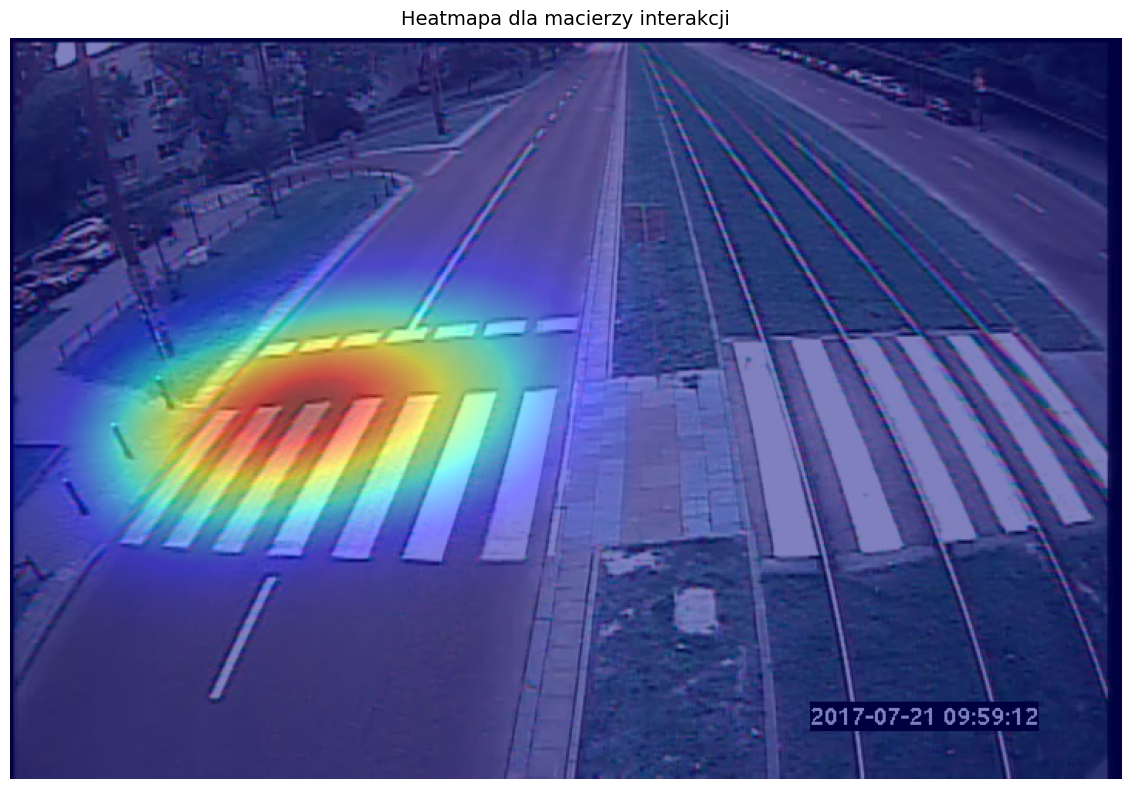
\includegraphics[width=0.95\textwidth]{images/film3/mapa7.png}
    \caption{Mapa ciepła wygenerowana dla macierzy interakcji pomiędzy obiektami klasy pojazdy i osoby dla nagrania nr 3}
\end{figure}
\begin{figure}[H]
    \centering
    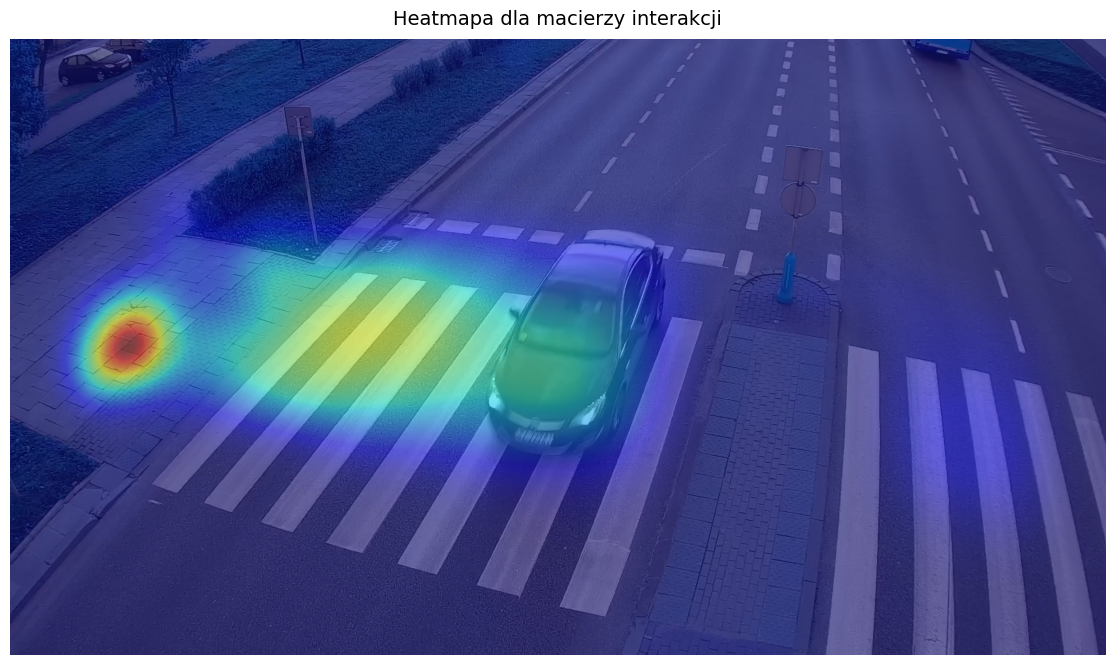
\includegraphics[width=0.95\textwidth]{images/film4/mapa7.png}
    \caption{Mapa ciepła wygenerowana dla macierzy interakcji pomiędzy obiektami klasy pojazdy i osoby dla nagrania nr 4}
\end{figure}
W celu dalszego wykorzystania w skrypcie selekcjonującym nagrania dla modelu wizualno-językowego notatnik dokonuje zapisu macierzy do pliku \textbf{interactionMatirx.npy}.
\section{Metody selekcji fragmentów nagrań i aktywacji modelu wizualno-językowego}
\label{sec:selekcja}
W fazie roboczej skrypt \textit{selekcja.py} wczytuje wygenerowaną wcześniej macierz interakcji i za pomocą detektora YOLO sprawdza czy w polu interkacji znajdują się obiekty należące do każdej z grup tzn. zarówno grupy pieszych (person, umberlla) oraz pojazdów (car, bus, truck, motorcycle). Jeśli tak to rozpoczynamy zapisywanie nagrania do pliku mp4. W momencie, gdy obiekt chociaż jednej z grup opuści pole interakcji, skrypt zaczyna odliczać 150 klatek do zakończenia nagrania o ile w polu interkacji nie pojawią się znowu obiekty obu interesujących nas grup. Każdy z plików zapisywany jest do folderu output pod nazwą output0, output1, ... Tak przygotowane nagranie może trafić na wejście modelu wizualno-językowego.
\begin{figure}[H]
    \centering
    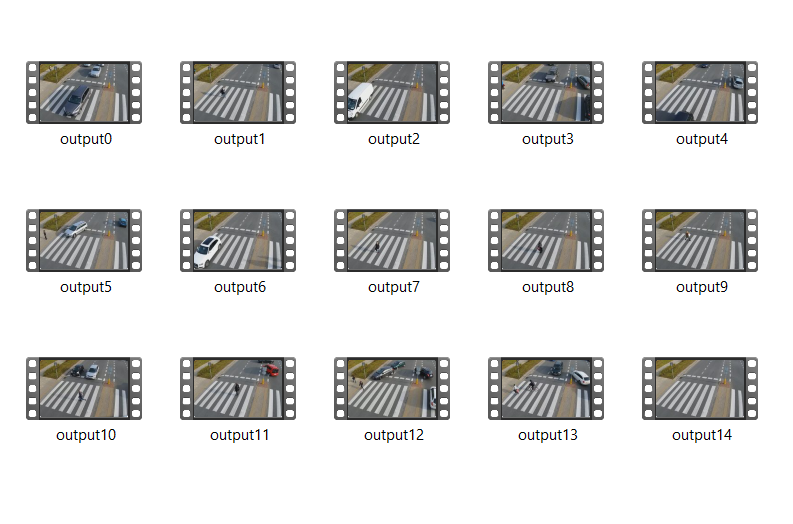
\includegraphics[width=0.95\textwidth]{images/nagrania.png}
    \caption{Przykładowe nagrania wyłuskane z filmu nr 1}
\end{figure}
\section{Podusmowanie, wnioski i dalsze kierunki badań}
Przedstawiony przeze mnie tryb manualny selekcji nagrań do modelu wizualno-językowego głównie ze względu na badany bardzo prosty klasyfikator Haara i prosty tracker centroidowy mierzył się w głównie z problemami z wykrywaniem obiektów jak również utrzymywaniem ich śledzenia. Wersja z YOLO naprawiała wiele z nich, jednakże ze względu na dążenie do automatyzacji całego procesu ta gałąź nie będzie miała dalszej kontynuacji w badaniach.

Dużo ciekawszym zagadnieniem był zdecydowanie tryb automatyczny detekcji. Tutaj w mojej ocenie osiągnięto dosyć ciekawe rezultaty dla różnych typów nagrań co pozwala mieć nadzieję, że sama metodyka analizy i selekcji nagrań jest trafna. Jak pokazały nagrania w fazie uczenia warto, aby nagrania były dosyć długie - w moim przypadku filmy godzinne pomimo gorszej jakości sprawdziły się lepiej niż filmy 15-minutowe. Dosyć prawidłowo na każdym z nagrań wykrywane były tory ruchu obiektów poszczególnych klas co pozwalało na sensowne wyznaczenie pól interakcji pomiędzy obiektami zgrupowanych klas. Uzyskane w rozdziale \ref{sec:selekcja} nagrania prezentują ciekawe zjawiska w ruchu drogowym jak i wiele sytuacji niebezpiecznych np. nieustąpienie pierwszeństwa przez samochody, wyprzedanie pojazdów przed przejściem dla pieszych w momencie gdy na przejściu znajduje się pieszy czy nagłe hamowania w celu przepuszczenia pieszych. W mojej ocenie takie fragmenty mogą się okazać bardzo przydatne w dalszych analizach z wykorzystaniem modeli wizualno-językowych.

W posiadanych przeze mnie nagraniach nie znajdował się żaden film nagrany w warunkach nocnych lub też innych problematycznych dla kamery np. w momencie gdy słońce oślepia kamerę lub jej część. W dalszych badaniach warto byłoby znaleźć takie nagrania i sprawdzić zachowanie się wypracowanych przeze mnie metod analizy. Ponadto domyślny tracker YOLO (BoT-SORT) gubi detekcje na nagraniach co może powodować zaburzenia w generowaniu map ciepła - korzystnym byłoby pochylenie się również nad tym zagadnieniem w dalszych pracach. Ponadto należy rozwiązać kwestię klasyfikacji detekcji, które na chwilę staną do klasy obiektów poruszających się. Tutaj warto byłoby zmienić sposób w jaki obiekty są przypisywane do obu klas z obecnej analizy średniego przemieszczenia na inny.

Podsumowując opracowana przeze mnie metodologia analizy nagrań z ruchu drogowego i selekcji interesujących fragmentów do dalszej analizy za pomocą modelu wizualno-językowego sprawdza się dosyć dobrze. Wstępna analiza nagrań pozwala rozpoznać tory ruchu pojazdów i ekstraktować interesujące fragmenty do przetwarzania przez model. Metoda choć wymaga poprawek już na obecnym etapie pozwala na dalszy rozwój projektu.
\section{Kody programów}
Wszystkie zamieszone tutaj kody znajdują się również w repozytorium \href{https://github.com/Lukasz004/VLM-traffic-analysis}{VLM-traffic-analysis} na platformie GitHub.
\subsection{wykrywanie\_haar.py}
\lstinputlisting[style=pythonStyle]{scripts/wykrywanie_haar.py}
\subsection{wykrywanie\_yolo.py}
\lstinputlisting[style=pythonStyle]{scripts/wykrywanie_yolo.py}
\subsection{video\_to\_json.py}
\lstinputlisting[style=pythonStyle]{scripts/video_to_json.py}
\subsection{aktywacja\_tracking.ipynb}
Plik notatnika aktywacja\_tracking.ipynb jest dostarczony w osobnym pliku.
\subsection{selekcja.py}
\lstinputlisting[style=pythonStyle]{scripts/selekcja.py}

\end{document}
